\documentclass[a4paper]{article}
\title{A Quick Introduction to TMM}
\author{Tatsuro Tanioka}
\date{\today}
% Recommended to compile with XeLaTeX

\usepackage[margin=1in]{geometry}
\usepackage{xcolor}
\usepackage{listings}
\lstdefinestyle{DOS}
{
    backgroundcolor=\color{black},
    basicstyle=\scriptsize\color{white}\ttfamily
}
\usepackage{natbib}
\usepackage{bibentry}
\nobibliography*
\usepackage{mathtools,amsthm}    % some advanced mathematics notation
\usepackage{graphicx}            % easy inclusion and manipulation of images
%\usepackage[draft]{graphicx}            % for draft- not displaying figures, comment out if display figures
\graphicspath{ {./Figures_tutorial/} }
\usepackage[font=small,labelfont=bf]{caption}
\usepackage{float}
\usepackage{microtype}           % just for fun: really hone in with the typography
\usepackage{booktabs}            % nice looking tables that present the content first and foremost
\usepackage{multicol}            % multiple columns in a local context
\usepackage[hidelinks]{hyperref} % clickable references in the output, but hide them visually
\usepackage{amssymb}
\usepackage{amsmath}
\usepackage[version=3]{mhchem}
\usepackage{newtxtext,newtxmath}
\usepackage{hyperref}
\usepackage{longtable}
\usepackage{enumitem}
\hypersetup{
    colorlinks=true,
    linkcolor=blue,
    filecolor=magenta,      
    urlcolor=cyan,
    citecolor=black,
%    pdftitle={Sharelatex Example},
%    bookmarks=true,
%    pdfpagemode=FullScreen,
    }
    
\urlstyle{same}

\def\noin{\noindent }
\def\CO{$\mathrm{CO_{2}}$ }
%%%%%%%%%%%%%----------------------------------------------------------
\begin{document}
\maketitle

\begin{abstract}
This document goes through how to use the Transport Matrix Model (TMM) using computational resources at the University of Minnesota's Minnesota Supercomputing Institution (MSI). All the source codes and documents (including this tutorial) that Tanioka made to TMM is available at my github website \url{(https://github.com/tanio003/tmm/tree/TT_Release)}.
\end{abstract}

\tableofcontents

\section{Setting up}

\subsection{Flow Chart}
Before you do anything, read ``README.txt'' by Samar Khatiwala at the following website: \\ \url{https://github.com/samarkhatiwala/tmm}. I will go over each of these steps specifically aimed at audiences using the computational cluster \emph{Mesabi}.
\begin{enumerate}
\item Installing and configuring PETSc
\item Downloading all the scripts and transport matrices into your own local directory
\item Compiling the model (we use the BGC model \verb/MOPS2/ for this example)
\item Running the model
\item Processing the model outputs
\item Displaying the model outputs
\end{enumerate}

\subsection{Steps}

\subsubsection{Step 0: Logging into MSI and Mesabi}
\noin Open the terminal (assuming that you have a MAC or Linux environment) on your computer and log in to MSI with your x500 account:
\begin{lstlisting}[style=DOS]
 $ ssh -Yt youremail@umn.edu
\end{lstlisting}

\noin Log in to Mesabi: 
\begin{lstlisting}[style=DOS]
 $ ssh -X mesabi
\end{lstlisting}

\noin Make a new directory called TMM2 in your home directory and enter into this directory. Everything related to TMM will go into this directory.
\begin{lstlisting}[style=DOS]
 $ mkdir TMM2
 $ cd TMM2
\end{lstlisting}

\subsubsection{Step 1: Installing and configuring PETSc}

\noin Download the latest version of PETSc and save it in your TMM2 directory and unzip this package. If opened properly, you should see the new directory petsc-3.13.5. 
\begin{lstlisting}[style=DOS]
 $ wget http://ftp.mcs.anl.gov/pub/petsc/release-snapshots/petsc-lite-3.13.5.tar.gz
 $ tar -xvf petsc-lite-3.13.5.tar.gz
 $ ls
 petsc-3.13.5
\end{lstlisting}

\noin Import the required modules: (1) impi, (2) impi/intel, and (3) cmake. Also make sure that you are using python 3, not python 2 (= default for MSI). 
\begin{lstlisting}[style=DOS]
 $ module purge 
 $ module load intel
 $ module load impi/intel
 $ module load cmake
 $ module load python3
 $ module list
Currently Loaded Modulefiles:
 1) intel/2018.release(default)   4) cmake/3.10.2(default)
 2) intel/2018/release            5) python3/3.7.1_anaconda
 3) impi/intel(default)
\end{lstlisting}

\noin Set up \verb/$PETSC_DIR/ to your petsc-3.13.5 directory. For your future uses, I would advise you to set \verb|$PETSC_DIR| in your \verb|.bashrc| as well. 
\begin{lstlisting}[style=DOS]
 $ export PETSC_DIR=$HOME/TMM2/petsc-3.13.5
 $ echo $PETSC_DIR 
 /.../TMM2/petsc-3.13.5
\end{lstlisting}

\noin Configure PETSc. Although this part is quite tricky you can copy and use my config file \\ ``\verb/reconfigure-arch-linux-c-opt.py/''. If the config file does not work properly, let me know and I can show you a way to compile without using this .py file. 
\begin{lstlisting}[style=DOS]
 $ cd petsc-3.13.5
 $ cp ~/../tanio003/TMM2/petsc-3.13.5/config/reconfigure-arch-linux-c-opt.py config/
 $ config/reconfigure-arch-linux-c-opt.py
\end{lstlisting}

\noin Don't worry about some warning signs. It takes few minutes to compile. If it's compiled properly you should see the notice ``Conifgure stage complete.'' Then build PETSc library:
\begin{lstlisting}[style=DOS]
 $ make all
\end{lstlisting}
Building process takes about 15-30 minutes. If you're very lucky it will go through in a single shot. But in most cases, it fails during the middle of the process. Don't worry if it fails the first time. Simply type ``\verb/$ make all/'' again and hopefully it will finish building from where it left off. If built properly, you should see the message ``Now to check if the libraries are working do:...''. Then type,
\begin{lstlisting}[style=DOS]
 $ make check
 ...
Completed test examples
\end{lstlisting}
If you get this far, you've managed to build the PETSc successfully and you're ready to go to the next step. If it failed, read the error messages, debug, and try again. \textbf{Building PETSc is harder than it looks} so you need to be patient. 

As more of a technical note, the procedure above uses the Intel compilers and Intel MPI library. By loading the cmake, the PETSc build system can learn more about the host machine. In addition to taking advantage of compiler optimizations and vectorization, the procedure above builds PETSc against the Intel Math Kernel Library (MKL) for BLAS, LAPACK and ScaLAPACK which gives a performance gain over the reference implementations. For the FORTRAN compiler, we specifically need to use \verb/mpiifort/, and not \verb/mpif90/ (the default compiler), because TMM codes are written in both F77 and F90. Also, since we don't require C++ for TMM we put the flag in the config file, \verb/--with-cxx=0/. The reason we need to use MPI compilers, not regular gcc compilers, is because we want to run PETSc in a parallel mode (i.e., by using the command \verb/mpiexec/ in the runscript). For more details about building PETSc please check out \url{https://www.mcs.anl.gov/petsc/documentation/installation.html}. 

\subsubsection{Step 2: Downloading all the scripts and transport matrices}
\begin{enumerate}
\item First download Matlab scripts from \\ 
\url{http://kelvin.earth.ox.ac.uk/spk/Research/TMM/tmm_matlab_code.tar.gz} and put into the first level of your TMM2 folder Path. You could also get my copy.
\begin{lstlisting}[style=DOS]
 $ cp -r ~/../tanio003/TMM2/tmm_matlab_code $HOME/TMM2/
\end{lstlisting}
\item Download transport matrices and related data for the model of your choice: \\ \url{http://kelvin.earth.ox.ac.uk/spk/Research/TMM/TransportMatrixConfigs/} and put into he first level of your TMM2 folder Path. You can download all 6 configurations but I warn you that \verb|MITgcm_ECCO_v4| and \verb|UVicKielIncrIsopycDiffTransient| take a very long time. For the ones that I have you could also grab my copy (e.g., to copy \verb|MITgcm_ECCO|):
\begin{lstlisting}[style=DOS]
 $ cp -r ~/../tanio003/TMM2/MITgcm_ECCO $HOME/TMM2/
\end{lstlisting}

\noin Alternatively, you can get download these TMM files from the web directly (e.g., to download \verb|MITgcm_ECCO|):
\begin{lstlisting}[style=DOS]
 $ wget kelvin.earth.ox.ac.uk/spk/Research/TMM/TransportMatrixConfigs/MITgcm_ECCO.tar
 $ tar -xvf MITgcm_ECCO.tar
\end{lstlisting}

\item Download miscellaneous data called OceanCarbon from \\ 
\url{http://kelvin.earth.ox.ac.uk/spk/Research/TMM/MiscData/}. You can get my copy by:
\begin{lstlisting}[style=DOS]
 $ cp -r ~/../tanio003/TMM2/OceanCarbon $HOME/TMM2/
\end{lstlisting}
\item Download source codes for TMM and models:
\begin{lstlisting}[style=DOS]
 $ git clone https://github.com/tanio003/tmm
\end{lstlisting}
 This directory (\verb|/TMM2/tmm|) contains the source codes from Khatiwala's master branch (``\verb|master|'') and my public release branch (``\verb|TT_Release|''). For our exercise, we will be using some of my new codes so you need to switch from the master branch to my branch in the newly created tmm directory:
\begin{lstlisting}[style=DOS]
 $ cd tmm
 (master) $ ls
 driver  HOWTO.txt  LICENSE.txt  models  README.txt
 (master) $ git checkout TT_Release
 (TT_Release) $ ls
 driver  HOWTO.txt  LICENSE.txt  models  README.txt  Tutorial_MSI
\end{lstlisting}
Notice that in the branch \verb|TT_Release|, there is a new directory \verb|Tutorial_MSI|, which was not present in the master branch. 

(Optional) If you want to make start making your own changes to the source codes, I would suggest making a new branch in your local computer (e.g.., \verb|yournewrepo|), and leave \verb|master| and \verb|TT_Release| untouched.
\begin{lstlisting}[style=DOS]
 (TT_Release) $ git checkout -b yournewrepo
 (yournewrepo) $ git branch --show-current
 yournewrepo
\end{lstlisting}
\item Set the environment variable TMMROOT to point to the top level of the TMM directory.
\begin{lstlisting}[style=DOS]
 (TT_Release) $ export TMMROOT=$HOME/TMM2/tmm
 (TT_Release) $ echo $TMMROOT
 /home/.../TMM2/tmm
\end{lstlisting}

For your future convenience, I would advise you to set \verb|$TMMROOT| in your \verb|.bashrc| as well so you don't need to set the variable every time you log in to MSI. 

\item To synchronize your \verb|tmm| folder with the remote repository (e.g., syncing \verb|TT_Release| with my updates), use the git pull command your terminal. I suggest you do this regularly to keep your files up to date.
\begin{lstlisting}[style=DOS]
 $ cd $TMMROOT
 $ git checkout TT_Release
 $ git pull origin TT_Release
\end{lstlisting}

\end{enumerate}

\subsubsection{Step 3: Compiling the model}
\noin Here, let's try compiling the biogeochemical MOPS. If you want to learn about the basic architecture of MOPS, read the model description paper by \citet{Kriest15} at \url{https://gmd.copernicus.org/articles/8/2929/2015/}. 

\begin{enumerate}
\item For each model there are model-specific source codes in the directory (\verb|$TMMROOT/models/current/mops2/|) and we need to import some of them to the run directory. First, we create a new run directory. I make a new base directory called ``\verb|Runs|'' and in that directory, I make subdirectories for specific experiments. I call it \verb|Runs/MOPS/Test_spinup| and copy here all the files needed.

\begin{lstlisting}[style=DOS]
 $ cd ~/TMM2
 $ mkdir -p Runs/MOPS/Test_spinup
 $ cd Runs/MOPS/Test_spinup
 $ cp -p $TMMROOT/models/current/mops2.0/src/Makefile .
 $ cp -p -R $TMMROOT/models/current/mops2.0/matlab/* .
 $ cp -p $TMMROOT/models/current/mops2.0/runscripts/* .
 $ cp -p $TMMROOT/models/current/mops2.0/parameters/* .
\end{lstlisting}

\item Compile mops. Make sure that all the modules are loaded and \verb|$PETSC_DIR| is set correctly before you compile mops.
\begin{lstlisting}[style=DOS]
 $ module load intel
 $ module load impi/intel
 $ module load cmake
 $ make cleanall
 $ make mops
\end{lstlisting}

\noin If compiled properly, you'd find a new executable ``mops'' created along with a bunch of objective .o files. 
\lstset{emph={mops,runscript_msi,Makefile}, emphstyle=\color{green}}
\begin{lstlisting}[style=DOS]
 $ ls
 BGC_INI.o                           n7fluxes28.m
 BGC_MODEL.o                         n7physics.m
 CAR_CHEM.o                          n7tracers28.m
 CAR_INI.o                           n7tracersavg28.m
 external_forcing_mops_biogeochem.o  perry1996-runoff-noarctic_noname.txt
 insolation.o                        perry1996-runoff_noname.txt
 load_output.m                       petsc_matvec_utils.o
 load_output_time_avg.m              petsc_signal_utils.o
 load_pco2.m                         process_output.m
 Makefile                            runscript
 make_input_files_for_mops_model.m   runscript_msi
 make_rivers.m                       tmm_external_bc.o
 misfit_mops_biogeochem.o            tmm_forcing_utils.o
 mops                                tmm_forward_step.o
 mops_biogeochem_copy_data.o         tmm_main.o
 mops_biogeochem_diagnostics.o       tmm_monitor.o
 mops_biogeochem_ini.o               tmm_profile_utils.o
 mops_biogeochem_misfit.o            tmm_timer.o
 mops_biogeochem_model.o             tmm_write.o
 mops_biogeochem_set_params.o        biogem_params.txt
\end{lstlisting}
\lstset{emph={}, emphstyle=\color{green}}

\item Edit the file \ \verb/make_input_files_for_mops_model.m/. First thing to do is to make sure that variable \verb/base_path/ point to the right directory for the TMM configuration.
\lstset{language=matlab} 
\begin{lstlisting}[frame=single,basicstyle=\scriptsize,commentstyle=\color{blue}]
 % make_input_files_for_mops_model.m
 
 % Set toplevel path to GCMs configuration
 % base_path='/data2/spk/TransportMatrixConfigs/MITgcm_2.8deg';
 % base_path='/data2/spk/TransportMatrixConfigs/MITgcm_ECCO';
 % base_path='/data2/spk/TransportMatrixConfigs/MITgcm_ECCO_v4';
 base_path='~/TMM2/MITgcm_2.8deg';
  %base_path='~/TMM2/MITgcm_ECCO';
  
 addpath(genpath('~/TMM2/tmm_matlab_code'));% add tmm_matlab_code to the search path
 oceanCarbonBasePath='~/TMM2/OceanCarbon';  % add OceanCarbon to the search path
 atmosDataPath=fullfile(oceanCarbonBasePath,'AtmosphericCarbonData');
\end{lstlisting}
\noin In the same matlab file, there are different switches (0 = no and 1 = yes). For this spin-up exercise, we \textbf{couple MOPS to a simple OCMIP-like carbon model} and \textbf{fix atmospheric $\mathrm{pCO_{2}}$ at 280 ppm}. So set the switches as following:
\begin{lstlisting}[frame=single,basicstyle=\scriptsize,commentstyle=\color{blue}]
 % make_input_files_for_mops_model.m
 ...
 periodicForcing=1 
 periodicMatrix=1
 
 dt=43200; % time step to use (43200s for ECCO and MIT2.8; 28800s for any other TMMs)
 
 rearrangeProfiles=1
 bigMat=0
 writeFiles=1
 writeTMs=1
 useCoarseGrainedMatrix=0
 writePCFiles=0
 
 READ_SWRAD=0                    % Read short-wave radiation?
 useCarbon=1                     % Use simple inorganic carbon model?
 useOrgCarbon=0                  % Use organic carbon module?
 useAtmModel=0                   % Use prognostic 1-box atmosphere?
 pCO2atm_ini=280.0               % Initial pco2?
 useTimeVaryingPrescribedCO2=0   % Use prescribed pco2 pathway?
 useVirtualFlux=1                % Use DIC and Alk to calculate E-P?
 empScaleFactor=1.0              % Scaling factor for E-P (default = 1)
 %-----------------------------------
 % Modified by Tatsuro Tanioka 200907 to allow for Atmospheric CO2 option
 % For a prescribed pCO2 run, useTimeVaryingPrescribedCO2=1 and choose a scenario
 
 % Available options: 'historical', 'RCP3PD', 'RCP45', 'RCP6' and 'RCP85'
 co2Scenario='RCP85';
 %-----------------------------------
\end{lstlisting}
\noin Then open MATLAB and run \verb/make_input_files_for_mops_model.m/
\begin{lstlisting}[style=DOS]
 $ module load matlab
 $ matlab -nodesktop
                                    < M A T L A B (R) >
                          Copyright 1984-2019 The MathWorks, Inc.
                     R2019a Update 5 (9.6.0.1174912) 64-bit (glnxa64)
                                      July 31, 2019
To get started, type doc.
For product information, visit www.mathworks.com.

>> make_input_files_for_mops_model
\end{lstlisting}
\noin This creates a bunch of periodic forcing files (\verb|xxx_01, xxx_02,...|), initial tracer concentrations \\ (\verb|po4ini.petsc, no3ini.petsc,...|), and binary files (.bin and .petsc) related to model geometry and forcing.

\item Edit the parameter file.  \verb|biogem_params.txt|. We only need to set the \textbf{first 7 parameters} because we are not using organic carbon module for this exercise. We will use the calibrated values for MOPS/MIT2.8 follwiing \cite{Kriest20}.

\lstset{language=sh} 
\begin{lstlisting}[frame=single,basicstyle=\scriptsize,commentstyle=\color{blue}]
  1.39     #01. detmartin = Martin Curve exponent of Detritus [1.39 for MIT2.8, 1.46 for ECCO]
  173.7    #02. ro2ut = Refield -O2:P                         [173.7 for MIT2.8, 151.1 for ECCO]
  0.00119  #03. nfix = Max growth rate (1/d) of N-fixers      [0.00119 for MIT2.8, 0.00229 for ECCO]
  15.8     #04. subdin = No denitrification below this level of DIN (mmol/m3)           [15.8, 16.0]
  1.01     #05. ACkbaco2 = Half sat-constant for oxic degradation (mmol/m3)             [1.01, 1.07]
  32.0     #06. ACkbacdin = Half sat-constant for suboxic degradation                   [32.0, 23.1]
  0.001    #07. alimit = Min. value for the degradation of PHY and DOP [0.001 for mops, 0.01 for mops_cp]
\end{lstlisting}

\end{enumerate}

\subsubsection{Step 4: Running the model}
\noin MSI systems use job queues to efficiently and fairly manage when computations are executed. The queuing system at MSI is called Slurm and to submit a job to a queue users create Slurm job scripts. The script contains information on the resources requested for calculation, as well as the commands for executing the calculation. 

Below is the custom Slurm script for submitting a new job to run MOPS2 using Mesabi. It's called \verb|runscript_msi| and should be in the current directory already.

\lstset{language=sh} 
\begin{lstlisting}[frame=single,basicstyle=\scriptsize]
#!/bin/bash -l        
#SBATCH --nodes=1
#SBATCH --ntasks-per-node=24
#SBATCH --mem-per-cpu=2gb
#SBATCH --time=06:00:00
#SBATCH --mail-type=ALL  
#SBATCH --mail-user=tatsurobkkuk@gmail.com
#SBATCH -p small
#SBATCH --output=%j.out

cd $SLURM_SUBMIT_DIR

module load intel
module load impi/intel
module load cmake
\end{lstlisting}

\noin The first line defines which type of shell the script will be read. Here we will use the \verb|bash|. Commands for the Slurm queuing system begin with \verb|#SBATCH|. Lines 2 to 4 in the above sample script contain the Slurm resource request. The current job will require about 6 hours, 1 node each with 24 processor cores, and 2GB of memory per core . The two lines containing \verb|#SBATCH --mail| are both commands having to do with sending message emails to the user. The first of these lines instructs the Slurm system to send a message email when the job aborts, begins, or ends. The second command specifies the email address to be used. Using the message emails is recommended because the reason for a job failure can often be determined using information in the emails. A Slurm script should contain the appropriate change directory commands to get to the job execution location. A Slurm script also needs to contain module load commands for any software modules that the calculation might need. 

The follwing lines (17$\sim$) in \verb|runscript_msi| contain the commands to execute and start a specific program. Different flags need to be change accordingly depending on the nature of experiments. For more information on different options available, read ``HOWTO.txt'' by S. Khatiwala located in \verb|$TMMROOT|. Do not put these  \verb|#| comments in the actual file. 

\lstset{language=sh} 
\begin{lstlisting}[frame=single,basicstyle=\scriptsize,commentstyle=\color{blue}]
# 360 days per year with a time step of 2 steps per day:
mpirun -np 24 ./mops \ # number of cores, models
        -numtracers 9 \  # number of tracers (i.e. state variables)
        -i po4ini.petsc,dopini.petsc,oxyini.petsc,phyini.petsc,zooini.petsc,detini.petsc,no3ini.petsc,
        dicini.petsc,alkini.petsc \  # files for initialization of BGC state variables
        -me Ae \   # the name of the explicit transport matrix
        -mi Ai \   # the name of the implicit transport matrix
        -t0 0.0 -iter0 0 \
        -deltat_clock 0.0013888888888889 \  # starting time[years] starting time[timesteps]: for initial run
        -max_steps 2160000 \   # total number of timesteps to be evaluated (here 3000 yrs)
        -write_time_steps 72000 \   # output frequency(in timesteps, here every 100 yrs)
        -o po4out.petsc,dopout.petsc,oxyout.petsc,phyout.petsc,zooout.petsc,detout.petsc,no3out.petsc,
        dicout.petsc,alkout.petsc \   # files for output of 9 BGC state variables
        -external_forcing \   # calculate BGC explicitly
        -use_profiles \
        -nzeuph 2 \   # number of layers in euphotic zone (2 for MIT2.8, 6 for ECCO)
        -biogeochem_deltat 43200.0 -days_per_year 360.0 \ # ocean timestep[seconds]
        -burial_sum_steps 720 \  # sum burial over a period of 720 timesteps = 1 yr
        -pco2atm 280.0 \ # use fixed pCO2 of 280 ppm
        -use_virtual_flux \ # use the global surface mean DIC and Alk to calculate E-P
        -periodic_matrix \ # use of periodic transport matrix # the unit of time is year and 
 # circulation has a periodicity of 1 year; monthly mean tranport matrix (12 TMs/year)
        -matrix_cycle_period 1.0 -matrix_num_per_period 12 \
        -periodic_biogeochem_forcing \
        -periodic_biogeochem_cycle_period 1.0 -periodic_biogeochem_num_per_period 12 \
        -num_biogeochem_steps_per_ocean_step 8 \  # the number of BGC timestep per ocean step
        -separate_biogeochem_time_stepping \ # timestep BGC model separately from ocean step
        -time_avg -avg_start_time_step 2159281 -avg_time_steps 60 \
        # initial timestep for diagnostic fluxes (for final year); avg over 60 timesteps = 1 month
        -avg_files po4avg.petsc,dopavg.petsc,oxyavg.petsc,phyavg.petsc,zooavg.petsc,detavg.petsc,no3avg.petsc,
        dicavg.petsc,alkavg.petsc \ # avg file names
        -bgc_params_file biogem_params.txt \   # parameter files to be read
        -num_bgc_params 7 \   # number of parameters read
        -calc_diagnostics -diag_start_time_step 2159281 -diag_time_steps 60 \
        # initial timestep for diagnostic fluxes (for final year); avg over 60 timesteps = 1 month
        -diag_files fbgc1.petsc,fbgc2.petsc,fbgc3.petsc,fbgc4.petsc,fbgc5.petsc,fbgc6.petsc,fbgc7.petsc,
        fbgc8.petsc \ # diagnsotic flux files names
        > log # outputting to logfile

 \end{lstlisting}

\noin Currently BGC model writes the following 8 diagnostics into the different files:
\begin{enumerate}
\item \verb|fbgc1.petsc|: primary production in each box [$\mathrm{mmol P/m^3/oceantimestep}$]
\item \verb|fbgc2.petsc|: zooplankton grazing in each box  [$\mathrm{mmol P/m^3/oceantimestep}$]
\item \verb|fbgc3.petsc|: detritus sedimentation through upper boundary of \\ each box  [$\mathrm{mmol P/m^2/oceantimestep}$]
\item \verb|fbgc4.petsc|: remineralization of detrius and DOP in each box [$\mathrm{mmol P/m^3/oceantimestep}$]
\item \verb|fbgc5.petsc|: river runoff  [$\mathrm{mmol P/m^3/oceantimestep}$]
\item \verb|fbgc6.petsc|: nitrogen fixation  [$\mathrm{mmol N/m^3/oceantimestep}$]
\item \verb|fbgc7.petsc|: denitrification  [$\mathrm{mmol N/m^3/oceantimestep}$]
\item \verb|fbgc8.petsc|: Irradiance at the top of every layer in euphotic zone [$\mathrm{W/m^2}$], added by T.Tanioka (2020/11)
\end{enumerate}

\noin To submit the job to the queue, type on the command line:
\begin{lstlisting}[style=DOS]
 $ chmod u+x runscript_msi
 $ sbatch runscript_msi
\end{lstlisting}

\noin To check your job status at MSI, type:
\begin{lstlisting}[style=DOS]
 $ squeue -u yourusername
\end{lstlisting}

\subsubsection{Step 5: Processing the model outputs}

\noin When the run is completed, you should receive an email from MSI (if you set it so in the runscript). You should also check you log file and the bottom of the log file should say ``Wall clock time xxx seconds''. As the output files are binary and cannot be opened on its own, we have to convert from the binary format into either netcdf (.nc) or Matlab (.mat) files using Matlab scripts.

\vspace{5mm}
\noin (Option 1, recommmended): To convert to \textbf{.nc} files you are going to use the following 5 scripts:
\begin{enumerate}
\item \verb|n7tracers28.m|: This file converts each tracer snapshot .petsc file (e.g., po4put.petsc) into a single .nc file. The MATLAB syntax is:
\begin{lstlisting}[style=DOS]
 >> n7tracers28('filename1.nc')
\end{lstlisting}
Make sure to set the basepath correctly and set useCarbon=1 (when carbon model is used) and useOrgCarbon=0. Also make sure that there is no .nc file with the same name already in the directory.

\item\verb|n7tracersavg28.m|: This file converts each tracer time-averaged .petsc file (e.g., po4avg.petsc) into a single .nc file. The MATLAB syntax is:
\begin{lstlisting}[style=DOS]
 >> n7tracersavg28('filename2.nc')
\end{lstlisting}
Make sure to set the basepath correctly and set useCarbon=1 and useOrgCarbon=0.

\item\verb|n7fluxes28.m|: This file converts each diagnostic flux .petsc file (e.g., fbgc1.petsc) into a single .nc file. The MATLAB syntax is:
\begin{lstlisting}[style=DOS]
 >> n7fluxes28('filename3.nc')
\end{lstlisting}
Make sure to set the basepath correctly and and set useOrgCarbon=0.

\item\verb|n7physics.m|: This file makes single .c files with monthly mean temperature and salinity. The MATLAB syntax is:
\begin{lstlisting}[style=DOS]
 >> n7physics('filename4.nc')
\end{lstlisting}
Make sure to set the basepath correctly and make sure that there is no .nc file with the same name already in the directory.

\item\verb|load_pco2.m|: This file makes a global mean atmospheric $\mathrm{pCO_{2}}$ file (``pco2.nc'') and surface $\mathrm{CO_{2}}$ air-sea flux file (``co2airseaflux.nc''). $\mathrm{CO_{2}}$ is in ppm and $\mathrm{CO_{2}}$ air-sea flux is in [$\mathrm{mmol C/m^2/timestep}$] (positive flux means $\mathrm{CO_{2}}$ is going into the sea from air). The MATLAB syntax is 
\begin{lstlisting}[style=DOS]
 >> load_pco2
\end{lstlisting}
Make sure to set the basepath and the $\mathrm{CO_{2}}$ run options correctly.

\item\verb|process_output.m| (optinal): To run all 5 scripts at once, edit and use this file. The MATLAB syntax is 
\begin{lstlisting}[style=DOS]
 >> process_output
\end{lstlisting}

\end{enumerate}

\noin (Option 2): To convert to \textbf{.mat} files you are going to run 2 scripts:
\begin{enumerate}

\item \verb|load_output.m|: This file converts each tracer snapshot .petsc file (e.g., po4put.petsc) to .mat file. Make sure to edit the \verb|base_path| and add \verb|tmm_matlab_code| to search path in lines 2 and 3.
\item \verb|load_output_time_avg.m|: This file converts each tracer average concentration .petsc file (e.g., po4avg.petsc) to .mat file. Make sure to edit the \verb|base_path| and search path correctly.
\item Unfortunately I don't have scripts for creating .mat diagnostic flux files, physics files, and $\mathrm{CO_{2}}$ files. But this should not be too hard to do and all you have to do is to modify other .m files.

\end{enumerate}

\subsubsection{Step 6: Displaying the model outputs}
\noin (Option 1): To view .nc files, I recommend the software \emph{Ferret} developed by NOAA. It is already installed in MSI, and to launch Ferret, type on the command line:
\begin{lstlisting}[style=DOS]
 $ ls *.nc
 filename1.nc filename2.nc filename3.nc filename4.nc co2airseaflux.nc pco2.nc
 $ module load ferret/7.6.0
 $ ferret
 	NOAA/PMEL TMAP
 	PyFerret v7.6 (optimized)
 	Linux 4.15.0-1089-azure - 06/25/20
 	11-Nov-20 16:51

yes? load filename1.nc
yes? sho d
     currently SET data sets:
    1> ./filename1.nc  (default)
 name     title                             I         J         K         L
 PO4                                       1:128     1:64      1:15      1:31
 DOP                                       1:128     1:64      1:15      1:31
 OXYGEN                                    1:128     1:64      1:15      1:31
 PHYTO                                     1:128     1:64      1:15      1:31
 ZOO                                       1:128     1:64      1:15      1:31
 DET                                       1:128     1:64      1:15      1:31
 NO3                                       1:128     1:64      1:15      1:31
 DIC                                       1:128     1:64      1:15      1:31
 ALK                                       1:128     1:64      1:15      1:31
\end{lstlisting}
I won't go into too much detail here but to learn more about Ferret, visit NOAA's website and take a tutorial at \url{https://ferret.pmel.noaa.gov/Ferret/documentation/ferret-tutorials}. You can make all kinds of graphs and figures with Ferret.

\vspace{5mm}
\noin (Option 2): If you want to visualize .mat files, I recommend the MATLAB package \verb|m_map|. Again, I would not go into much detail here but if you want to learn about it, download the package and take the tutorial from the developer's website: \url{https://www.eoas.ubc.ca/~rich/map.html}. Compared to Ferret, you have more freedom for customizing graphs. The downside is that you are going to have to write much longer codes.

\section{Case Studies}
\subsection{Study 1: Postindustrial $\mathrm{CO_{2}}$ uptake with MOPS+MIT2.8}
\noin In the first case study, we will simulate postindustrial $\mathrm{CO_{2}}$ uptake using MOPS and MITgcm2.8 under IPCC's RCP8.5 scenario from 1765 to 2265. We are going to do the continuous run from the spinup run (Section 1) so make sure that you have completed that run before you proceed.
\begin{enumerate}

\item Update source codes in your \verb|tmm| directly by doing \verb|git pull| from the remote repository.
\begin{lstlisting}[style=DOS]
 $ cd $TMMROOT
 $ git checkout TT_Release
 $ git pull origin TT_Release
\end{lstlisting}

\item Make a new run directory. Let's call it \verb|Test_co2historyRCP85| and copy all the files needed into this directory.
\begin{lstlisting}[style=DOS]
 $ cd ~/TMM2
 $ mkdir -p Runs/MOPS/Test_co2historyRCP85
 $ cd Runs/MOPS/Test_co2historyRCP85
 $ cp -p $TMMROOT/models/current/mops2.0/src/Makefile .
 $ cp -p -R $TMMROOT/models/current/mops2.0/matlab/* .
 $ cp -p $TMMROOT/models/current/mops2.0/runscripts/* .
  $ cp -p $TMMROOT/models/current/mops2.0/parameters/* .
\end{lstlisting}

\item Compile mops as we have done in the spinup run. Don't forget to load modules and make sure that environmental variables \verb|$TMMROOT| and \verb|$PETSC_DIR| are set up properly.
\begin{lstlisting}[style=DOS]
 $ make cleanall
 $ make mops
\end{lstlisting}

\item Copy the file \verb|pickup.petsc| from the spinup run directory into the current working directory and give it a new name (restart.petsc). This petsc files contains the tracer concentrations from the final year of the run and is required for the continuous run.

\begin{lstlisting}[style=DOS]
 $ cp ../Test_spinup/pickup.petsc restart.petsc
\end{lstlisting}

\noin Also, copy the file \verb|pickup_runoff.bin| from the spinup run directory. This binary file contains the global sedimentation from the final year of the previous run.
\begin{lstlisting}[style=DOS]
 $ cp ../Test_spinup/pickup_runoff.bin restart_runoff.bin
\end{lstlisting}

\noin (Optional) Instead of copying files, you can also create symbolink links so that you would know exactly where these restart files actually come when you do \verb|$ls -l|.
\begin{lstlisting}[style=DOS]
 $ ln -s ../Test_spinup/pickup.petsc restart.petsc
 $ ln -s ../Test_spinup/pickup_runoff.bin restart_runoff.bin
 $ ls -l restart.petsc
 lrwxrwxrwx. 1 tanio003 matsumot 26 Sep 28 12:33 restart.petsc -> ../Test_spinup/pickup.petsc
\end{lstlisting}

\item Edit the input generation file (\verb|make_input_files_for_mops_model.m|). The key here is to set \\ \verb|useTimeVaryingPrescribedCO2=1| and choosing the appropriate \verb|co2Scenario|, in this case RCP85. 
\lstset{language=matlab} 
\begin{lstlisting}[frame=single,basicstyle=\scriptsize,commentstyle=\color{blue}]
 % make_input_files_for_mops_model.m
 
 % Set toplevel path to GCMs configuration
 % base_path='/data2/spk/TransportMatrixConfigs/MITgcm_2.8deg';
 % base_path='/data2/spk/TransportMatrixConfigs/MITgcm_ECCO';
 % base_path='/data2/spk/TransportMatrixConfigs/MITgcm_ECCO_v4';
 base_path='~/TMM2/MITgcm_2.8deg';
 %base_path='~/TMM2/MITgcm_ECCO';
 
 addpath(genpath('~/TMM2/tmm_matlab_code'));% add tmm_matlab_code to the search path
 oceanCarbonBasePath='~/TMM2/OceanCarbon';  % add OceanCarbon to the search path
 atmosDataPath=fullfile(oceanCarbonBasePath,'AtmosphericCarbonData');
 ...
  
 READ_SWRAD=0                    % Read short-wave radiation?
 useCarbon=1                     % Use simple inorganic carbon model?
 useOrgCarbon=0                  % Use organic carbon module?
 useAtmModel=0                   % Use prognostic 1-box atmosphere?
 pCO2atm_ini=280.0               % Initial pco2? (will be ignored as useAtmModel=0)
 useTimeVaryingPrescribedCO2=1   % Use prescribed pco2 pathway?
 useVirtualFlux=1                % Use DIC and Alk to calculate E-P?
 empScaleFactor=1.0              % Scaling factor for E-P (default = 1)
 %-----------------------------------
 % Modified by Tatsuro Tanioka 200907 to allow for Atmospheric CO2 option
 % For a prescribed pCO2 run, useTimeVaryingPrescribedCO2=1 and choose a scenario
 
 % Available options: 'historical', 'RCP3PD', 'RCP45', 'RCP6' and 'RCP85'
 co2Scenario='RCP85';
 %-----------------------------------
\end{lstlisting}

\item Open Matlab and make input files:
\begin{lstlisting}[style=DOS]
 $ matlab -nodesktop
 ...
 >> make_input_files_for_mops_model
\end{lstlisting}

\item Edit \verb|runscript_msi|. Important changes are commented with blue (do not actually put these comments after line 13 on the script). You can manually edit the script or copy my script from \\ \verb|~/../tanio003/TMM2/Runs/MOPS/Testruns/Slurm/Test_co2historyRCP85_slurm|.
\lstset{language=sh} 
\begin{lstlisting}[frame=single,basicstyle=\scriptsize,commentstyle=\color{blue}]
  1 #!/bin/bash -l
  2 #SBATCH --nodes=1
  3 #SBATCH --ntasks-per-node=24
  4 #SBATCH --mem-per-cpu=2gb
  5 #SBATCH --time=00:60:00
  6 #SBATCH --mail-type=ALL
  7 #SBATCH --mail-user=tatsurobkkuk@gmail.com
  8 #SBATCH -p small
  9 #SBATCH --output=%j.out
 10
 11 cd $SLURM_SUBMIT_DIR
 12
 13 module load intel
 14 module load impi/intel
 15 module load cmake
 16
 17 # 360 days per year with a time step of 2 steps per day:
 18 mpirun -np 24 ./mops \
 19   -numtracers 9 \
 20   -pickup restart.petsc \   # read initial values from file
 21   -me Ae \
 22   -mi Ai \
 23   -t0 1765.0 -iter0 0 \   # start from year 1765
 24   -deltat_clock 0.0013888888888889 \   
 25   -max_steps 360000 \  # run for 720*500 timesteps = 500 years
 26   -write_time_steps 7200 \   # output every 720*10 timestep = 10 years
 27   -o po4out.petsc,dopout.petsc,oxyout.petsc,phyout.petsc,zooout.petsc,
 detout.petsc,no3out.petsc,dicout.petsc,alkout.petsc \
 28   -external_forcing \
 29   -use_profiles \
 30   -nzeuph 2 \
 31   -biogeochem_deltat 43200.0 -days_per_year 360.0 \
 32   -burial_sum_steps 720 \
 33   -runoff_ini_file restart_runoff.bin \ # read global sedimentation of previous run
 34   -periodic_matrix \
 35   -pco2atm_history TpCO2.bin,pCO2atm.bin \ # read prescribed pCO2 and time
 36   -use_virtual_flux \
 37   -matrix_cycle_period 1.0 -matrix_num_per_period 12 \
 38   -periodic_biogeochem_forcing \
 39   -periodic_biogeochem_cycle_period 1.0 -periodic_biogeochem_num_per_period 12 \
 40   -num_biogeochem_steps_per_ocean_step 8 \
 41   -separate_biogeochem_time_stepping \
 42   -time_avg -avg_start_time_step 169201 -avg_time_steps 720 \ 
 # output annual avg. from year 2000 (235 years after 1765)
 43   -avg_files po4avg.petsc,dopavg.petsc,oxyavg.petsc,phyavg.petsc,zooavg.petsc,
 detavg.petsc,no3avg.petsc,dicavg.petsc,alkavg.petsc \
 44    -bgc_params_file biogem_params.txt \
 45     -num_bgc_params 7 \
 46   -calc_diagnostics -diag_start_time_step 169201 -diag_time_steps 720 \ 
 # output annual mean fluxes from 2000 (235 years after 1765)
 47   -diag_files fbgc1.petsc,fbgc2.petsc,fbgc3.petsc,fbgc4.petsc,fbgc5.petsc,
 fbgc6.petsc,fbgc7.petsc,fbgc8.petsc \
 48   > log
\end{lstlisting}

\item Make sure that paramter file (\verb|biogem_params.txt|) is same as the one used in the spinup run. You can simply copy that file into the current directory.
\begin{lstlisting}[style=DOS]
 $ cp ../Test_spinup/biogem_params.txt .
\end{lstlisting}

\item Submit the job to MSI queue.
\begin{lstlisting}[style=DOS]
 $ sbatch runscript_msi
\end{lstlisting}

\item Processing and outputting results. Use 5 Matlab scripts \\ (\verb|n7tracers28.m,n7tracersavg28.m,n7fluxes28.m,n7physics.m,load_pco2.m|) to create .nc files. Here, I will show you how to plot $\mathrm{CO_{2}}$ timeseries and global annual mean air-sea flux of $\mathrm{CO_{2}}$ using Ferret. The script is also at \\ \verb|~/../tanio003/TMM2/Runs/MOPS/Testruns/Slurm/Test_co2historyRCP85_slurm/analyzeoutput.jnl|. 
\begin{lstlisting}[style=DOS]
 $ module load ferret/7.6.0
 $ ferret
  	NOAA/PMEL TMAP
 	PyFerret v7.6 (optimized)
 	Linux 4.15.0-1089-azure - 06/25/20
 	16-Sep-20 14:49
 yes? use pco2.nc
 yes? use co2airseaflux.nc
 yes? set w 1;plot/d=1/hlimits=1800:2120/vlimits=200:1200/title="pCO2 RCP8.5" pco2
 yes? ppl XLAB Year
 yes? ppl YLAB pCO2 (ppm)
 yes? ppl PLOT
 yes? set w 2 ; sha/d=2/x=-180:180/lev=(-Inf)(-4,4,0.8)(Inf)/palette=cmocean_balance/
 title="Annual CO2 flux (mol C m-2 yr-1)" co2air_to_sea_flux[l=10]*2*360/1000*(-1);go fland
 yes? set w 3 ; sha/d=2/x=-180:180/lev=(-Inf)(-4,4,0.8)(Inf)/palette=cmocean_balance/
 title="Annual CO2 flux (mol C m-2 yr-1)" co2air_to_sea_flux[l=100]*2*360/1000*(-1);go fland
 yes? set w 4; plot/d=2/hlimits=2000:2100/vlimits=-7:0/
 title="Ocean-atmosphere CO2 flux (PgC yr-1)" co2air_to_sea_flux[x=@din,y=@din]*2*360/1000*12/1e15*(-1)
\end{lstlisting}

\begin{figure}[H]   % Insert Figure 1 here
   \centering
   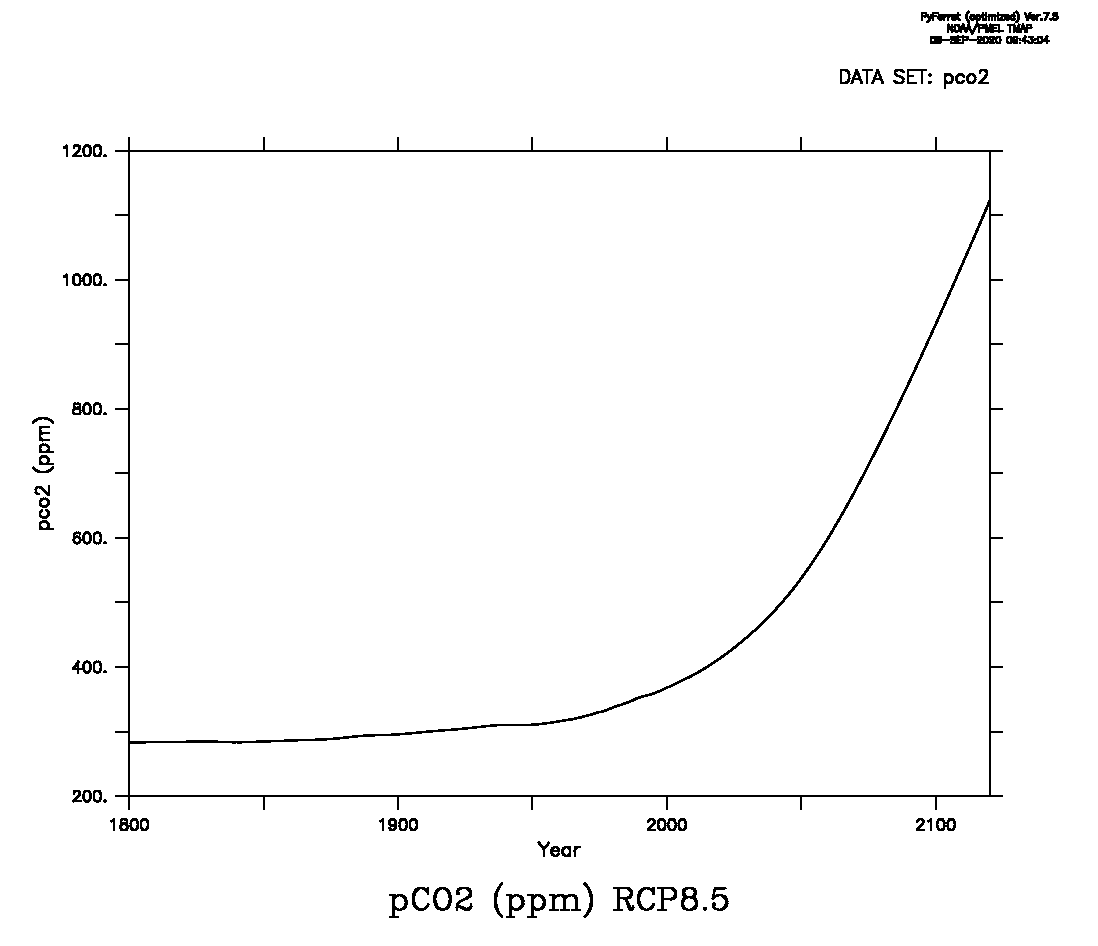
\includegraphics[width=10cm]{pco2RCP85.pdf}
   \caption[]{$\mathrm{CO_2}$ concentration pathway under RCP8.5 scenario \citep{Meinshausen11}.}
   \label{fig:pco2RCP85}
\end{figure}

Figure \ref{fig:pco2RCP85} (\emph{Ferret:w 1}) shows the change in $\mathrm{CO_2}$ under RCP8.5 scenario. There is a rapid increase in \CO concenctration from the late 1990s. 

Figure \ref{fig:airseamap} compares annual mean $\mathrm{CO_2}$ flux in 2010 (\emph{Ferret:w 2}) and 2100 (\emph{Ferret:w 3}). Notice that in 2010, large parts of the equatorial regions are net source of $\mathrm{CO_2}$ but in 2100, larger parts are becoming sink. Also, greater part of the Southern Ocean is also expected to absorb more  $\mathrm{CO_2}$ in 2100 compared to 2010. 

Figure \ref{fig:airseamapWoolf} is a $\mathrm{CO_2}$ flux in 2010 from a study by \cite{Woolf19} who used Surface $\mathrm{CO_2}$ atlas and wind data. If you compare with the left panel of Figure  \ref{fig:airseamap}, you can see that our MOPS model does a quite good job in reproducing the large scale pattern.

\begin{figure}[H]   % Insert Figure 2 here
   \centering
   \begin{minipage}{0.45\columnwidth}
      \centering
      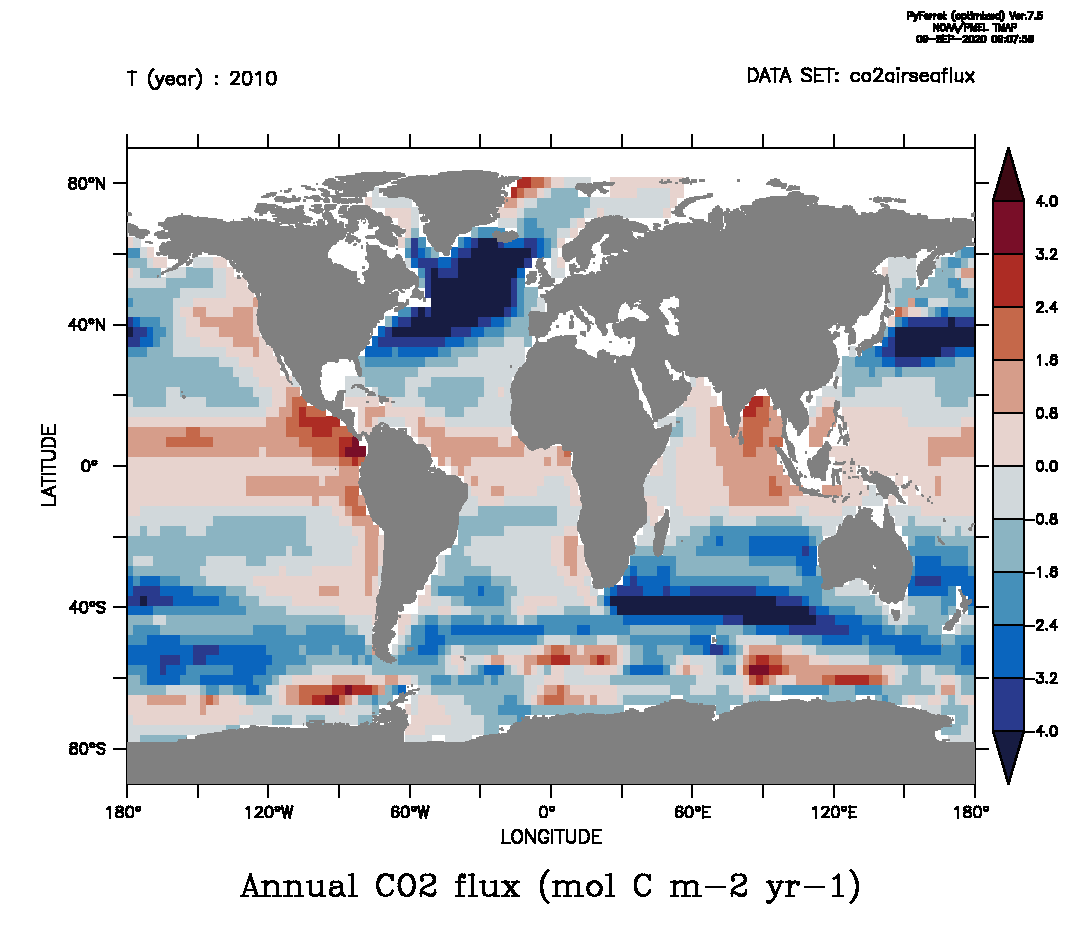
\includegraphics[width=\columnwidth]{airseaflux2010.pdf}
   \end{minipage}
   \begin{minipage}{0.45\columnwidth}
      \centering
      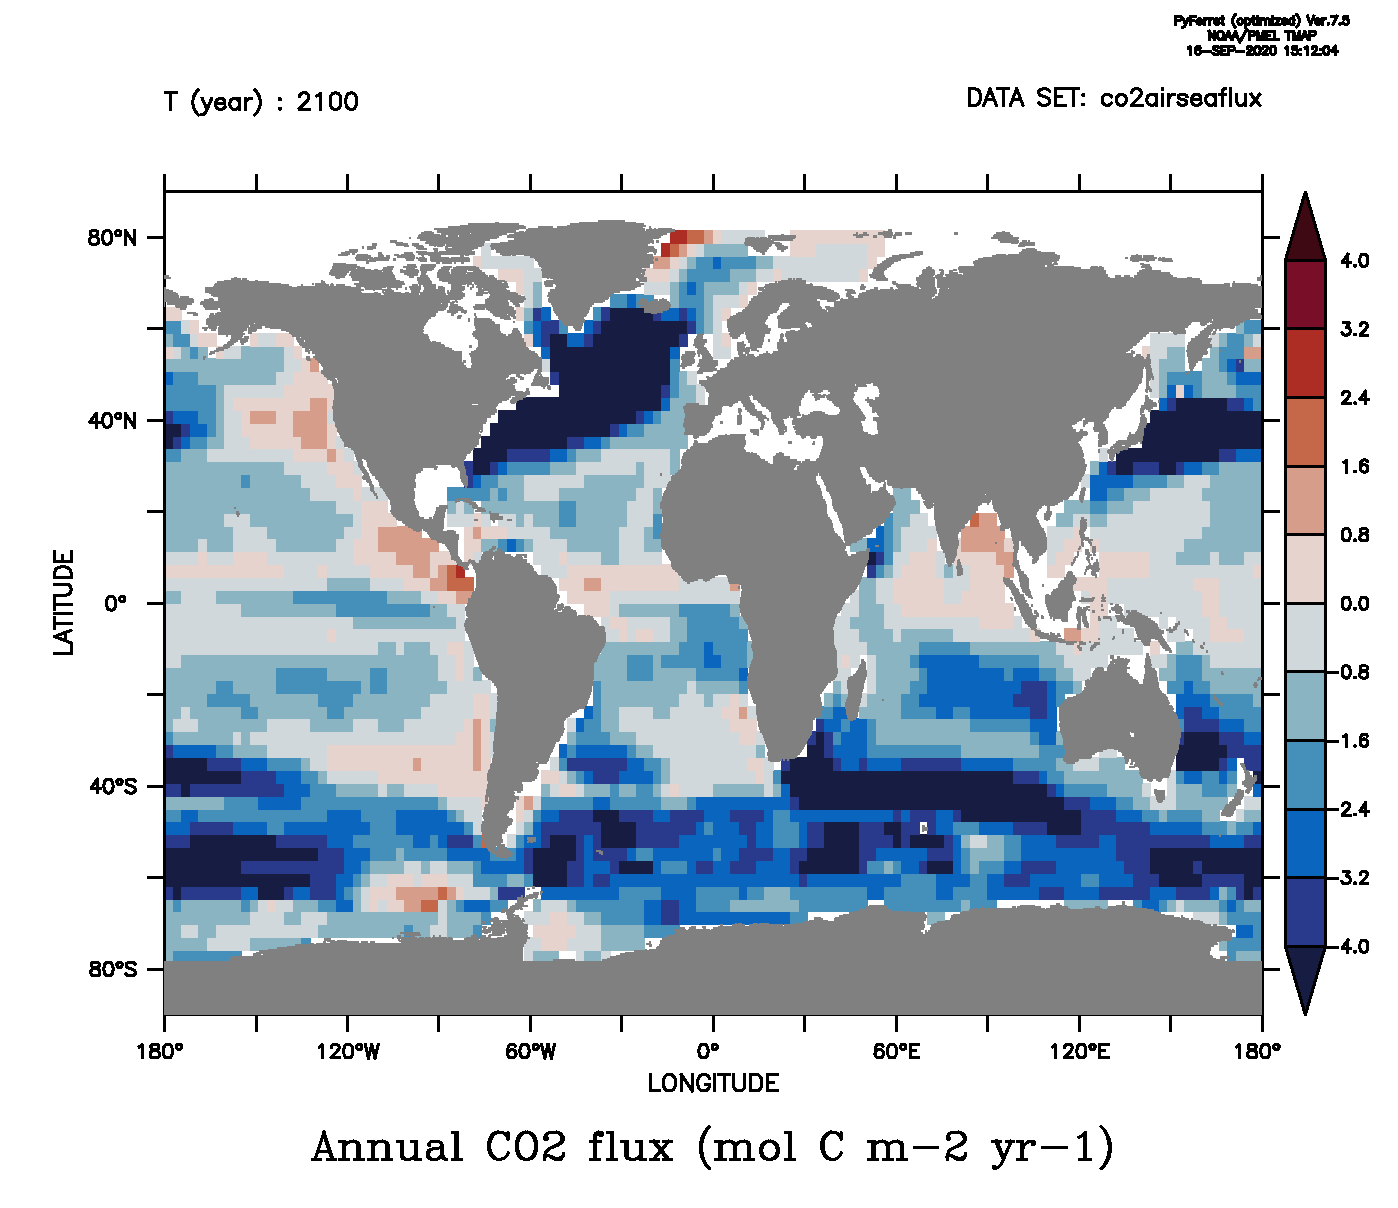
\includegraphics[width=\columnwidth]{airseaflux2100.pdf}
   \end{minipage}
   \caption[]{Modeled map of annual $\mathrm{CO_{2}}$ flux for 2010 (Left) and for 2100 (Right). Upward fluxes are defined as positive.}
   \label{fig:airseamap}
\end{figure}

\begin{figure}[h!]   % Insert Figure 3 here
   \centering
   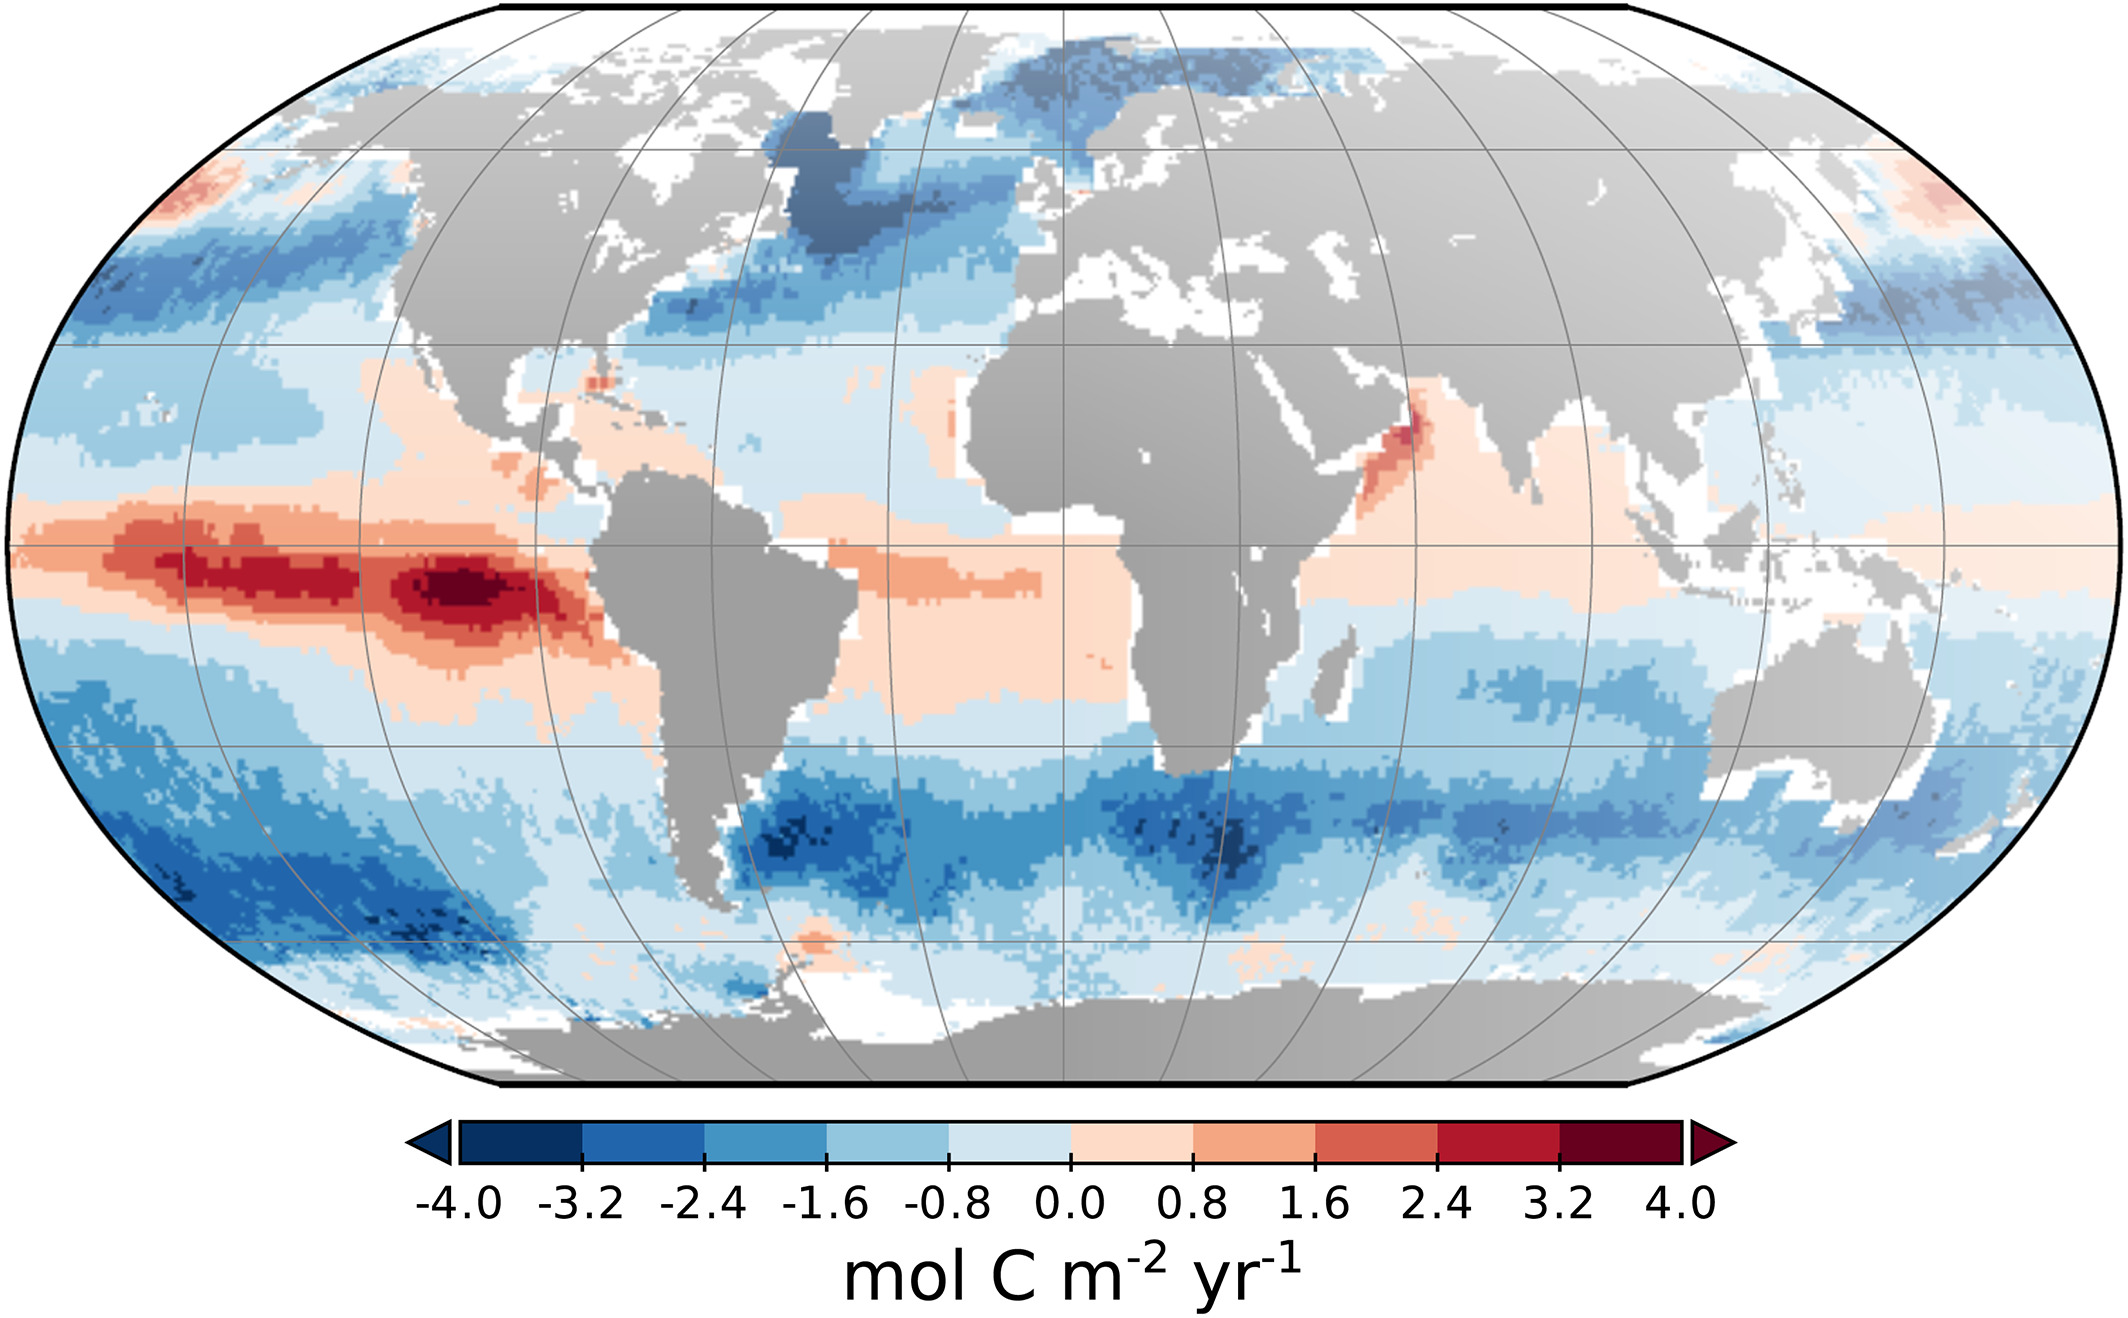
\includegraphics[scale=0.1]{Woolf19_GBC_Fig1.jpg}
   \caption[]{Map of annual $\mathrm{CO_{2}}$ flux in 2010 from $\mathrm{CO_2}$ and wind data \citep[from][]{Woolf19}. Compare this with Figure \ref{fig:airseamap}.}
   \label{fig:airseamapWoolf}
\end{figure}

Figure \ref{fig:airseatimeseries} (\emph{Ferret:w 4}) is a globally integrated sea-air $\mathrm{CO_2}$ flux projections under RCP8.5 scenario.The negative value means net uptake of $\mathrm{CO_2}$ by ocean. For a comparison, we show the similar projection using the CESM and CMIP5 (Figure \ref{fig:airseatimeseries_cmip5}a-b.) from \cite{Lovenduski16}. Again, notice that MOPS's result is largely consistent in terms of the magnitude. 

\begin{figure}[h!]   % Insert Figure 4 here
   \centering
   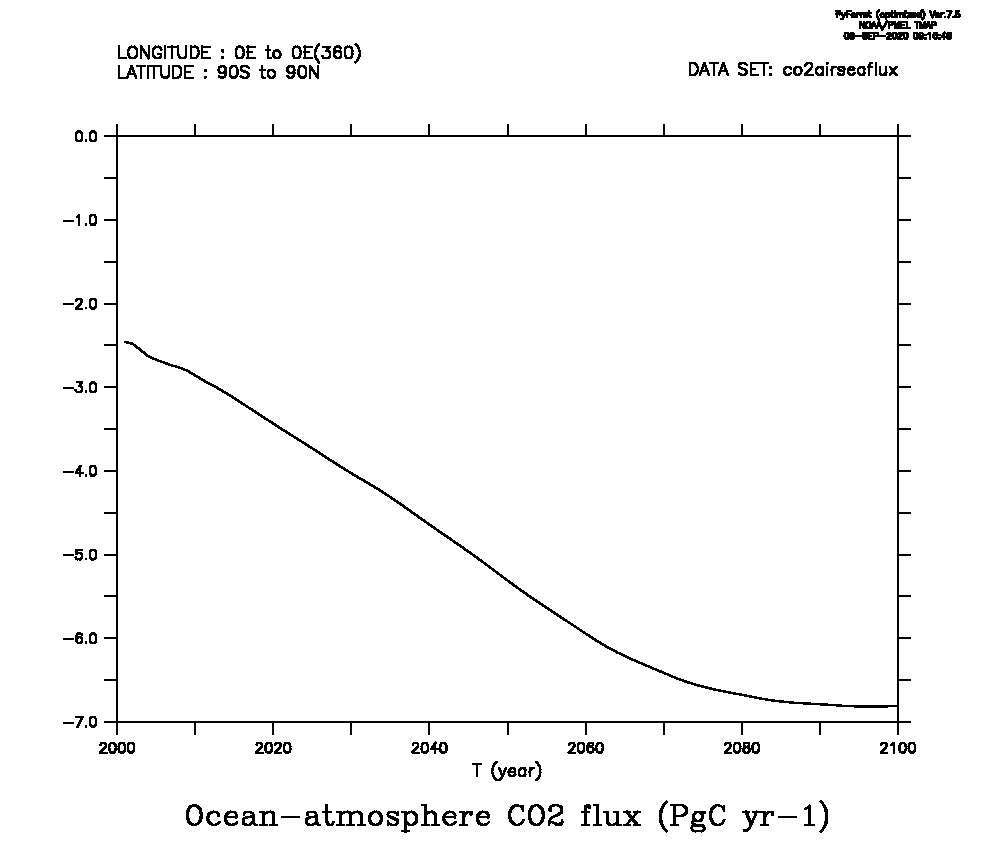
\includegraphics[scale=0.35]{airseaflux_timeseries2000to2100.pdf}
   \caption[]{Modeled annual-mean globally integrated sea-air $\mathrm{CO_2}$ flux projections under RCP8.5 scenario.}
   \label{fig:airseatimeseries}
\end{figure}

\begin{figure}[h!]   % Insert Figure 5 here
   \centering
   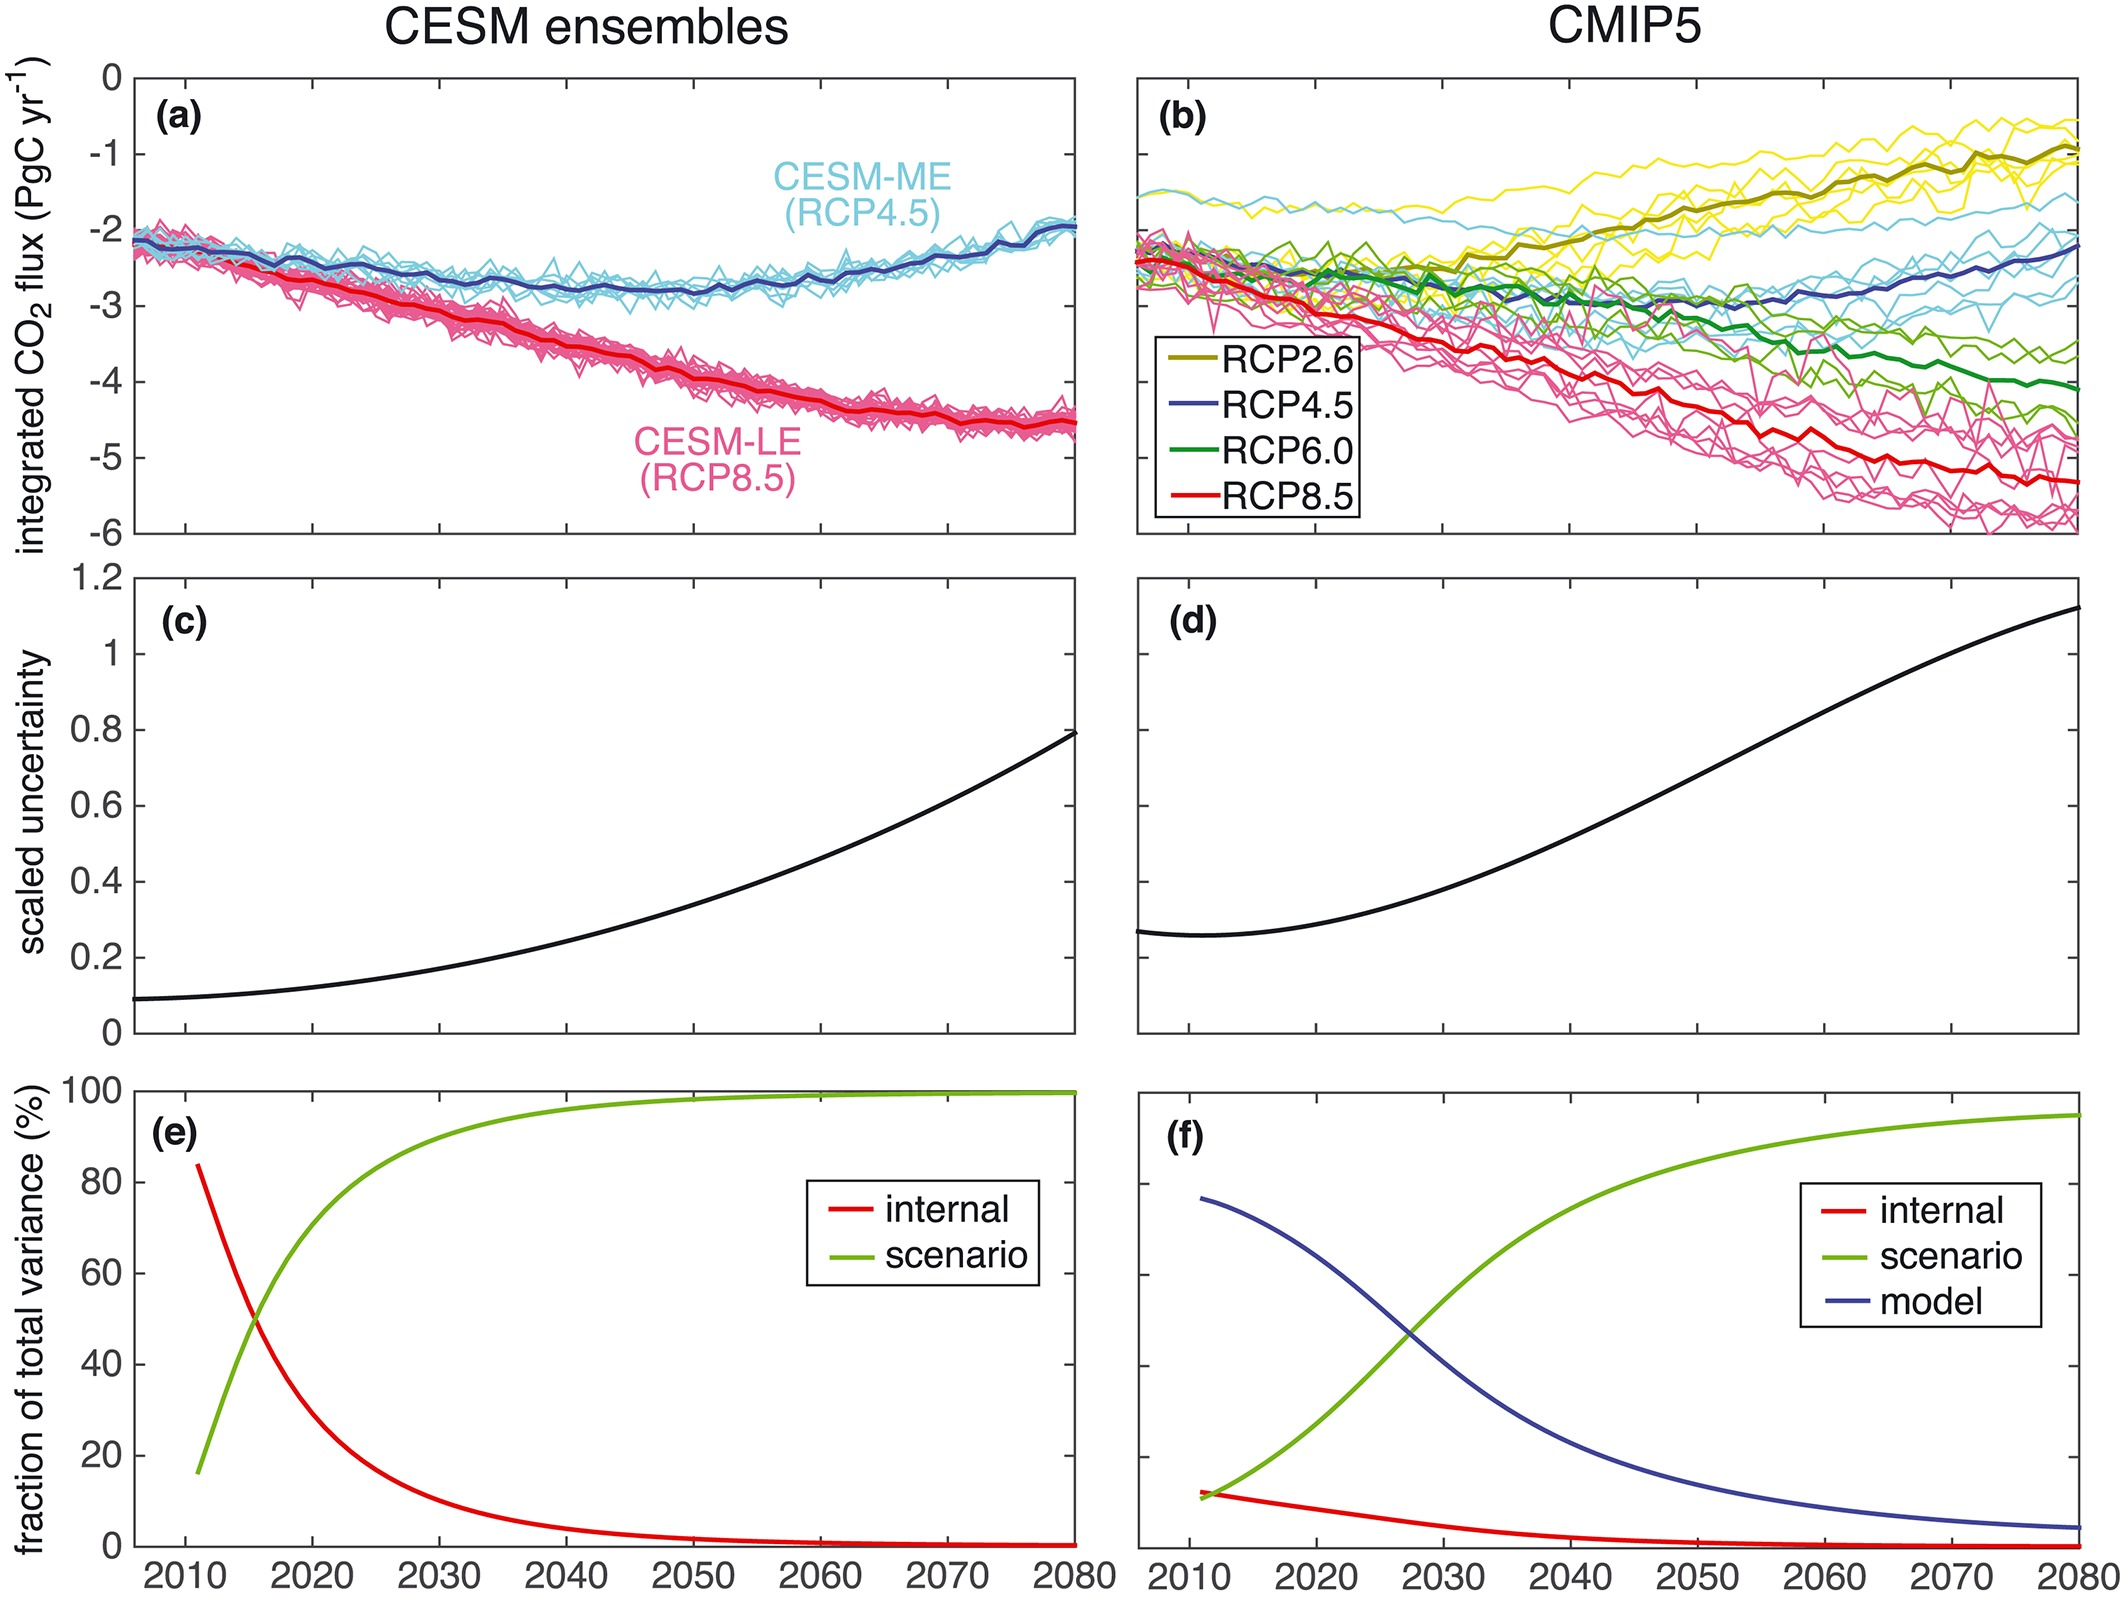
\includegraphics[trim=0 760 0 0,clip,scale=0.3]{Lovenduski16_GBC_Fig2.jpg}
   \caption[]{Modeled annual-mean globally integrated sea-air $\mathrm{CO_2}$ flux projections \citep[from][]{Lovenduski16} with CESM (a) and CMIP5 models (b). Compare this with Figure \ref{fig:airseatimeseries}.}
   \label{fig:airseatimeseries_cmip5}
\end{figure}

\end{enumerate}

\subsection{Study 2: Using MOPS+ECCO to simulate flexible C:P}

In the second case study, we will use the modified MOPS code to study the spatiotemporal variability in organic matter C:P ratio under steady-state scenario. We are going to do a  1000-yr spinup run where C:P of phytoplankton is flexible but C:P of zooplankton is homeostatic (i.e. less flexible). We will use the TMM model 12 monthly mean TMs derived from the Estimating the Circulation and Climate of the Ocean (ECCO) project, which provides circulation fields that yield a best fit to hydrographic and remote sensing observations over a 10-year period, on a spatial grid of 1-by-1 degree horizontal resolution with 23 vertical levels

We model P:C uptake ratio of phytoplankton using the power-law as a function of nutrients, temperature, and light following \cite{Tanioka20}:
\begin{equation}
   \mathrm{(P:C)_{uptake,phyto}} = \mathrm{(P:C)_{ref} \Bigl (\frac{[\ce{PO4}]}{[\ce{PO4}]_0} \Bigr )^{s^{P:C}_{PO_4}} \Bigl (\frac{[\ce{NO3}]}{[\ce{NO3}]_0} \Bigr )^{s^{P:C}_{NO_3}} \Bigl (\frac{[\ce{T}]}{[\ce{T}]_0} \Bigr )^{s^{P:C}_{T}} \Bigl (\frac{[\ce{I}]}{[\ce{I}]_0} \Bigr )^{s^{P:C}_{I}}} \label{eq:eq_pcphy}
\end{equation}
Exponent $\mathrm{{s^{P:C}_{driver}}}$ is constant and describe the strength of a given driver on P:C. 

Zooplankton P:C uptake ratio is also computed using the power-law as a function of phytoplankton P:C of biomass:
\begin{equation}
   \mathrm{(P:C)_{uptake,zoo}} = \mathrm{(P:C)_{ref,zoo}^{1-H}\cdot (P:C)_{biomass,phyto}^{H}} \label{eq:eq_pczoo}
\end{equation}

Parameter $H$ is a zooplankton homeostatic parameter that describes how variable zooplankton P:C is affected by phytoplankton P:C. When $H = 0$, P:C uptale equals a fixed reference P:C and is independent of phytoplankton P:C. When $H = 1$, uptake P:C equals cellular P:C of phytoplankton ("you are what you eat"). Here we will use the value of $H = 0.08$ following \cite{Persson10}, who conducted meta-analysis on zooplankton C:P.

In order to cope with the mismatch between required P:C and P:C of prey, zooplankton can excrete excess P or C as dissolved and particulate organic matter. In teh default setting, all the excess material will be routed towards particulate phase. This can be changed by adjusting the parameter \verb|par_excrtodoc| (default value = 0.0). At steady state, uptake P:C ratio should equal the biomass P:C ratio for both phytoplankton and zooplankton.

In implementing flexible C:P, I added 4 new tracers: (1) Phytoplankton C biomass, (2) Zooplankton C biomass. (3) DOC, and (4) POC. The total number of tracers is now 13. 

\begin{enumerate}
\item{Update source codes in your \verb|tmm| directly by doing \verb|git pull| from the remote repository.}
\begin{lstlisting}[style=DOS]
 $ cd $TMMROOT
 $ git checkout TT_Release
 $ git pull origin TT_Release
\end{lstlisting}

\item Make a new run directory. Here, we call it \verb|Test_ECCO_CP| and copy all the files needed into this directory. I also created a new directory called \verb|paramters| which contains an ASCII text file (\verb|biogem_params.txt|) with biogeochemical parameters.
\begin{lstlisting}[style=DOS]
 $ cd ~/TMM2
 $ mkdir -p Runs/MOPS/Test_ECCO_CP
 $ cd Runs/MOPS/Test_ECCO_CP
 $ cp -p $TMMROOT/models/current/mops2.0/src/Makefile .
 $ cp -p -R $TMMROOT/models/current/mops2.0/matlab/* .
 $ cp -p $TMMROOT/models/current/mops2.0/runscripts/* .
 $ cp -p $TMMROOT/models/current/mops2.0/parameters/* .
\end{lstlisting}

\item Compile mops. The new model with flexible C:P is called \verb|mops_cp|. 
\begin{lstlisting}[style=DOS]
 $ make cleanall
 $ make mops_cp
\end{lstlisting}

\item Edit the file \ \verb/make_input_files_for_mops_model.m/ and run it on Matlab. First thing to do is to make sure that variable \verb/base_path/ point to the right directory for the TMM ECCO configuration. Also make sure that option \verb|useORGCARBON| is set to 1. The options \verb|useORGCARBON| creates new initial concentrations arrays for DOC, POC, ZooC, and PhytoC. This initizalization process takes much longer than that of the first case study.

\noin (Optional) Instead of creating input matrix files each time, \textbf{you can create symbolic links} to the TMM matrices using the script "\verb|link_inputs.sh|" in the directory \verb|~/TMM2/tmm/models/current/mops2.0/runscripts|. This way it saves a lot of time and disc storage.

\item Edit the parameter input file \verb|biogem_params.txt|. In the first run, rows 1-6 should be the default values for MOPS + ECCO follwiing \cite{Kriest20}. Parameters 12-22 correspond to the P:C power-law formulations of phytoplankton and zooplankton from Equations (\ref{eq:eq_pcphy})-(\ref{eq:eq_pczoo}). Refernce P:C for both phytoplankton and zooplankton is $1/117 = 8.547$ permil (line 12). 
\begin{lstlisting}[frame=single,basicstyle=\scriptsize,commentstyle=\color{blue}]
  1 1.46     #01. detmartin = Martin Curve exponent of Detritus [1.39 for MIT2.8, 1.46 for ECCO]
  2 151.1    #02. ro2ut = Refield -O2:P                         [173.7 for MIT2.8, 151.1 for ECCO]
  3 0.00229  #03. nfix = Max growth rate (1/d) of N-fixers      [0.00119 for MIT2.8, 0.00229 for ECCO]
  4 16.0     #04. subdin = No denitrification below this level of DIN (mmol/m3)           [15.8, 16.0]
  5 1.07     #05. ACkbaco2 = Half sat-constant for oxic degradation (mmol/m3)             [1.01, 1.07]
  6 23.1     #06. ACkbacdin = Half sat-constant for suboxic degradation                   [32.0, 23.1]
  7 0.01     #07. alimit = Min. value for the degradation of PHY and DOP [0.001 for mops, 0.01 for mops_cp]
  8 1.46     #08. detmartin_c = Martin Curve Exponent of POC. For pref. remin, change from #01 [1.39, 1.46]
  9 1        #09. cp_option (1 = Power-law, 2: Galbraith and Martiny, 0: Redfield)
 10 250.0    #10. maxcp = upper bound C:P                                                 [250.0]
 11 50.0     #11. mincp = lower bound C:P                                                 [50.0]
 12 8.547    #12. par_bio_pc0 = Reference P:C (permil) for power-law                      [8.547]
 13 0.57     #13. par_bio_po4_ref = Reference PO4 (mmolP/m3) for power-law                [0.57]
 14 5.7      #14. par_bio_no3_ref = Reference NO3 (mmolN/m3) for power-law                [5.7]
 15 18.0     #15. par_bio_temp_ref = Reference Temp (deg C) for power-law                 [18.0]
 16 70.0     #16. par_bio_light_ref = Reference Irradiance (W/m2) for power-law           [70.0]
 17 0.21     #17. par_bio_spc_p = s_P:C^PO4 for power-law                                 [0.21]
 18 0.0      #18. par_bio_spc_n = s_P:C^NO3 for power-law                                 [0.0]
 19 0.0      #19. par_bio_spc_i = s_P:C^I for power-law                                   [0.0]
 20 -3.6     #20. par_bio_spc_t = s_P:C^T for power-law                                   [-3.6]
 21 0.08     #21. par_zoo_cp_hom = Homeostatic parameter for Zooplankton (0-1)            [0.08]
 22 0.0      #22. par_excrtodoc = Fraction of zooplankton adujstment flux going to DOC    [0.0]
\end{lstlisting}

\item Edit \verb|runscript_msi|. Here we are going to run the model for 15 hours with 10 nodes, 24 processors per core. Each processor is allocated with 2GB of memory. As we are using more than 9 nodes, we submit to the queue \textit{large}. If you want the job to proceed quicker, you can increase the number of nodes from 10. (Note: Asking for more nodes will mean longer time in the queue. So this will require some trial and error to find the optimal node request.)

Here is the first 12 lines of the runscript. The script is also at \\ \verb|~/../tanio003/TMM2/Runs/MOPS/Testruns_ECCO/201108b/runscript_msi|.
\lstset{language=sh} 
\begin{lstlisting}[frame=single,basicstyle=\scriptsize]
1 #!/bin/bash -l
2 #SBATCH --nodes=10
3 #SBATCH --ntasks-per-node=24
4 #SBATCH --mem-per-cpu=2gb
5 #SBATCH --time=15:00:00
6 #SBATCH --mail-type=ALL
7 #SBATCH --mail-user=tatsurobkkuk@gmail.com
8 #SBATCH -p large
9 #SBATCH --output=%j.out
10
11 cd $SLURM_SUBMIT_DIR
12
 \end{lstlisting}
 
The follwing lines (13$\sim$) contain the commands to execute and start the program \verb|mops_cp|. 

\lstset{language=sh} 
\begin{lstlisting}[frame=single,basicstyle=\scriptsize,commentstyle=\color{blue}]
 13 module load intel
 14 module load impi/intel
 15 module load cmake
 16
 17 # 360 days per year with a time step of 2 steps per day:
 18 mpirun -np 240 ./mops_cp \  # use 240=24*10 cores, program = mops_cp
 19         -numtracers 13 \   # use 13 tracers (9 tracers in mops + 4 new tracers)
 20         -i po4ini.petsc,dopini.petsc,oxyini.petsc,phyini.petsc,zooini.petsc,detini.petsc,
            no3ini.petsc,dicini.petsc,alkini.petsc,docini.petsc,pocini.petsc,phycini.petsc,
            zoocini.petsc \    # 13 initial tracer concentrations
 21         -me Ae \
 22         -mi Ai \
 23         -t0 0.0 -iter0 0 \
 24         -deltat_clock 0.0013888888888889 \
 25         -max_steps 2160000 \   # Run for 720 steps/year * 3000 years
 26         -write_time_steps 720000 \  # Output snapshot every 1000 years
 27         -o po4out.petsc,dopout.petsc,oxyout.petsc,phyout.petsc,zooout.petsc,detout.petsc,
            no3out.petsc,dicout.petsc,alkout.petsc,docout.petsc,pocout.petsc,phycout.petsc,
            zoocout.petsc \    # 13 output tracers 
 28         -external_forcing \
 29         -use_profiles \
 30         -nzeuph 6 \        # the default number of euphotic zones = 6 layers in ECCO 
 31         -biogeochem_deltat 43200.0 -days_per_year 360.0 \
 32         -burial_sum_steps 720 \
 33         -pco2atm 280.0 \   # Constant pCO2 at 280 ppm
 34         -use_virtual_flux \
 35         -periodic_matrix \
 36         -matrix_cycle_period 1.0 -matrix_num_per_period 12 \
 37         -periodic_biogeochem_forcing \
 38         -periodic_biogeochem_cycle_period 1.0 -periodic_biogeochem_num_per_period 12 \
 39         -num_biogeochem_steps_per_ocean_step 8 \
 40         -separate_biogeochem_time_stepping \
 41         -time_avg -avg_start_time_step 2159281 -avg_time_steps 60 \ # monthly avg in final year
 42         -avg_files po4avg.petsc,dopavg.petsc,oxyavg.petsc,phyavg.petsc,zooavg.petsc,detavg.petsc,
            no3avg.petsc,dicavg.petsc,alkavg.petsc,docavg.petsc,pocavg.petsc,phycavg.petsc,
            zoocavg.petsc \    # 4 new time-average tracers added 
 43         -bgc_params_file biogem_params.txt \   # telling to read the parameter file
 44         -num_bgc_params 22 \                   # the number of parameters to be read = 22
 45         -calc_diagnostics -diag_start_time_step 2159281 -diag_time_steps 60 \ # monthly diagnostics 
 46         -diag_files fbgc1.petsc,fbgc2.petsc,fbgc3.petsc,fbgc4.petsc,fbgc5.petsc,fbgc6.petsc,
            fbgc7.petsc,fbgc8.petsc,fbgc9.petsc,fbgc10.petsc,fbgc11.petsc \  # 11 diagnostics 
 47         > log
\end{lstlisting}
 
The important notes are commented with blue. The three new diagnostics related to organic carbon and flexible C:P module I added are: 
\begin{enumerate}
\item \verb|fbgc9.petsc|: POC sedimentation through upper boundary of each box [$\mathrm{mmol C/m^2/oceantimestep}$]
\item \verb|fbgc10.petsc|: Phytoplankton C:P uptake ratio in molar units.
\item \verb|fbgc11.petsc|: Zooplankton C:P uptake ratio in molar units.
\end{enumerate}
Monthly-averaged disgnostics as well as motnhly-averaged tracers will be computed in the final year (Year 2999) of the run.

\item To submit the job to the queue, type on the command line:
\begin{lstlisting}[style=DOS]
 $ chmod u+x runscript_msi
 $ sbatch runscript_msi
\end{lstlisting}

\noin To check your job status at MSI, type:
\begin{lstlisting}[style=DOS]
 $ squeue -u yourusername
\end{lstlisting}

\item Process the outputs using the Matlab Scripts as outlined previously. For each .m files \\
(\verb|n7tracers28.m,n7tracersavg28.m,n7fluxes28.m,n7physics.m,load_pco2.m|), 
make sure that variable \verb/base_path/ point to the right directory for the TMM ECCO configuration. Also make sure that option \verb|useORGCARBON| is set to 1.

\item Analyze outputs. Here we will look at seasonal cycles of productivity at 4 different locations. These 4 locations are: (1) the high latitude bloomforming North Atlantic Ocean (NAT: 25W-35W, 45N-50N, black line), (2) the North Atlantic subtropical gyre (NASG: 25W-70W, 25N-35N, red line), (3) the South Pacific subtropical gyre (SPSG:90W-150W, 15S-40S, green line), and (4) the Equatorial upwelling region (EQU: 5S-5N, blue line). The  code for making figrues is in my directory \\ \verb|~/../tanio003/TMM2/Runs/MOPS/Testruns_ECCO/201108b/analyze_201108b.jnl|.

Figure \ref{fig:mops_timeseries} shows the seasonal cycle of productivity (left) and the tracers/forcings (right). Notice that phytoplankton biomass exceeds zooplankton biomass throughout the year in all regions. The only exception is NAT where zooplankton biomass catches up with the phytoplankton biomass following the spring bloom. NPP peaks in early spring and export production lags NPP about a month or two. 

\begin{figure}[h!]   % Insert Figure 6 here
   \centering
   \begin{minipage}{0.495\columnwidth}
      \centering
      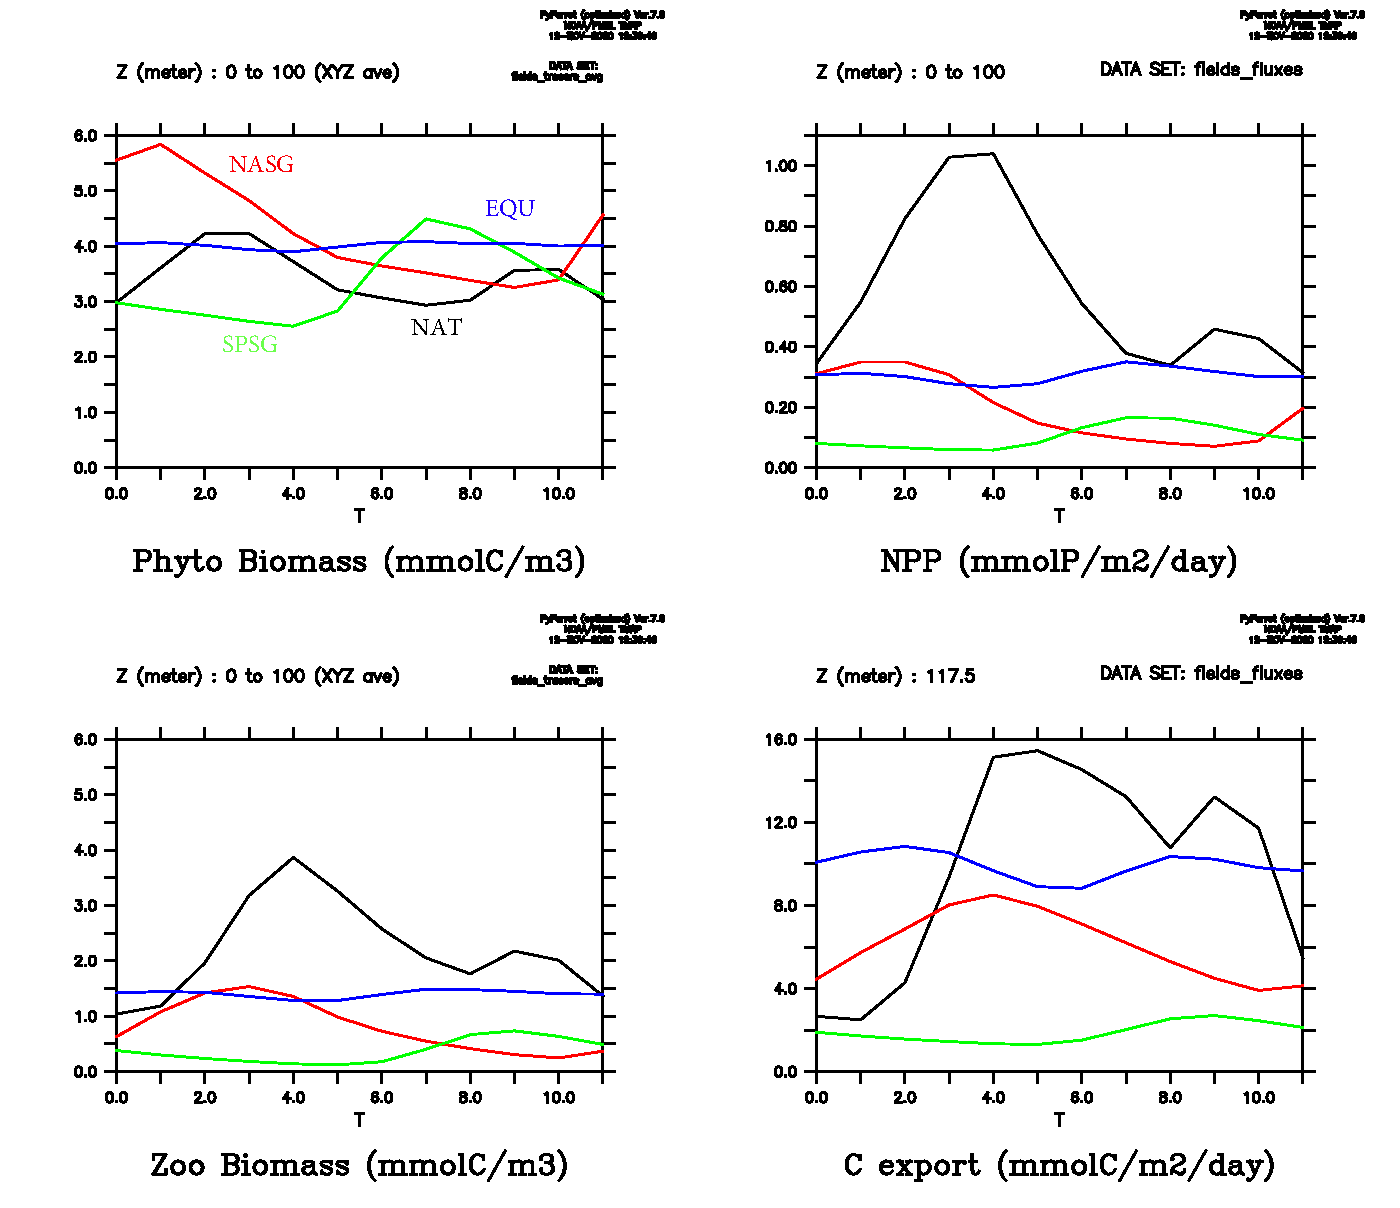
\includegraphics[width=\columnwidth]{productivity_comparison.pdf}
   \end{minipage}
   \begin{minipage}{0.495\columnwidth}
      \centering
      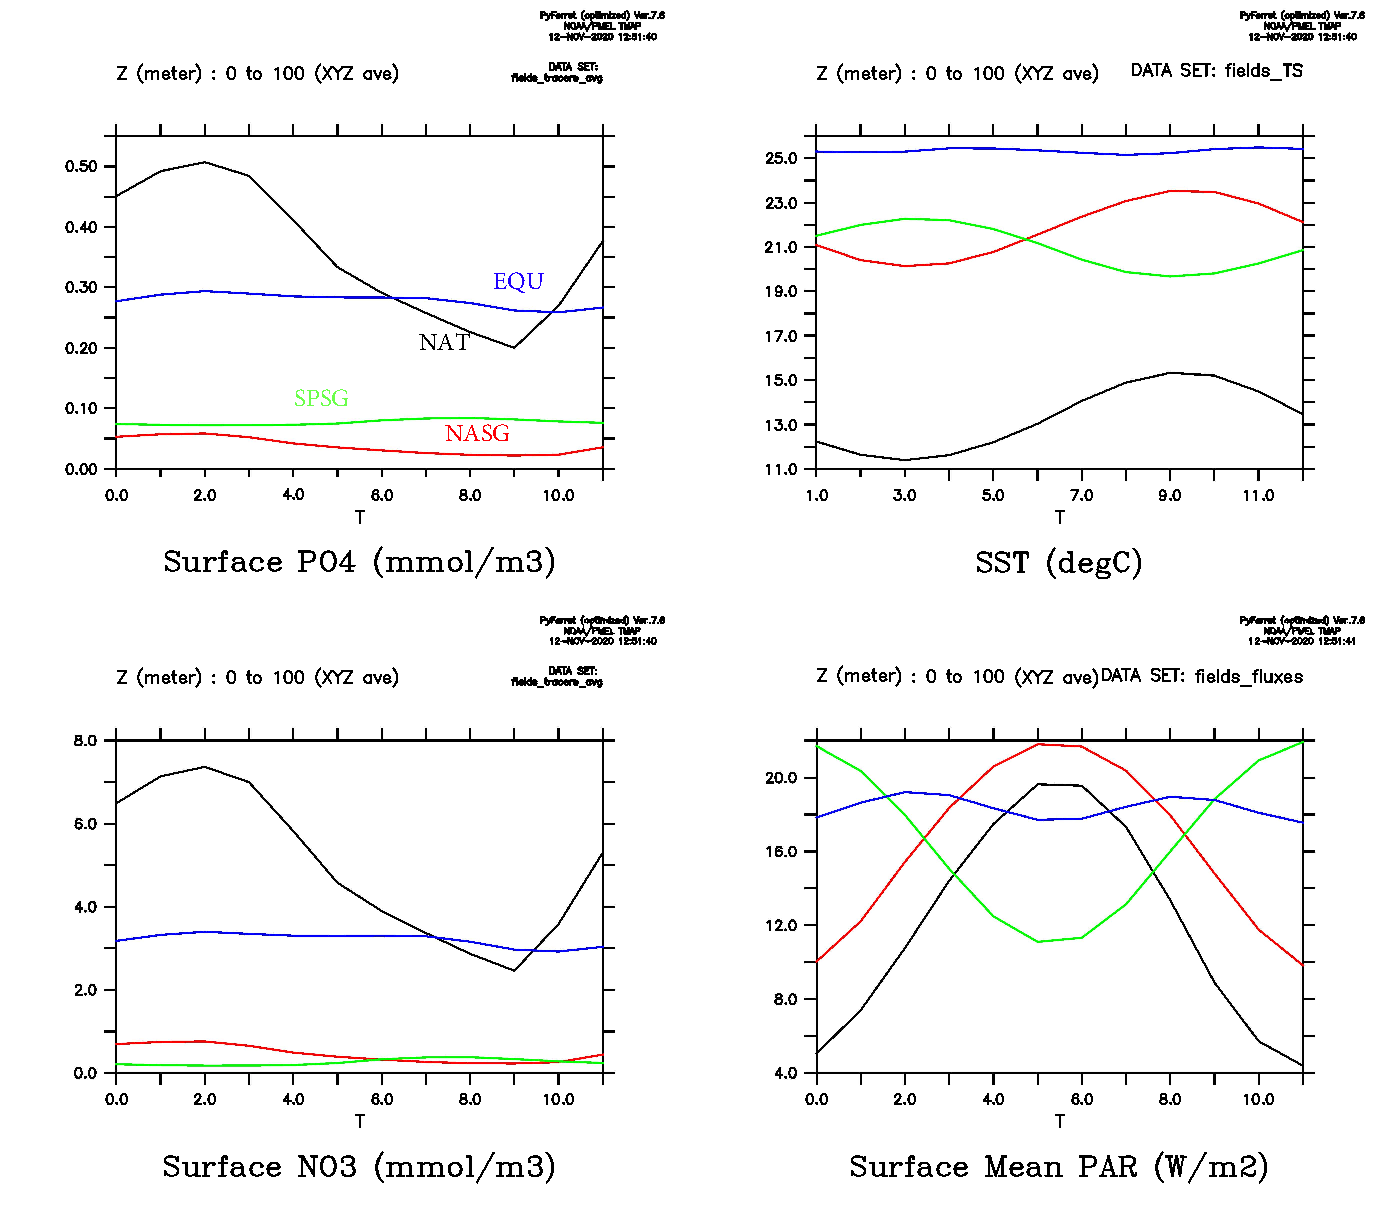
\includegraphics[width=\columnwidth]{driver_comparison.pdf}
   \end{minipage}
   \caption[]{Modeled seasonal cycle of productivity (Left) and tracers (Right) at four geographical regions. North Atlantic Ocean (NAT: 25W-35W, 45N-50N, black line), (2) the North Atlantic subtropical gyre (NASG: 25W-70W, 25N-35N, red line), (3) the South Pacific subtropical gyre (SPSG:90W-150W, 15S-40S, green line)}
   \label{fig:mops_timeseries}
\end{figure}

\begin{figure}[h!]   % Insert Figure 7 here
   \centering
   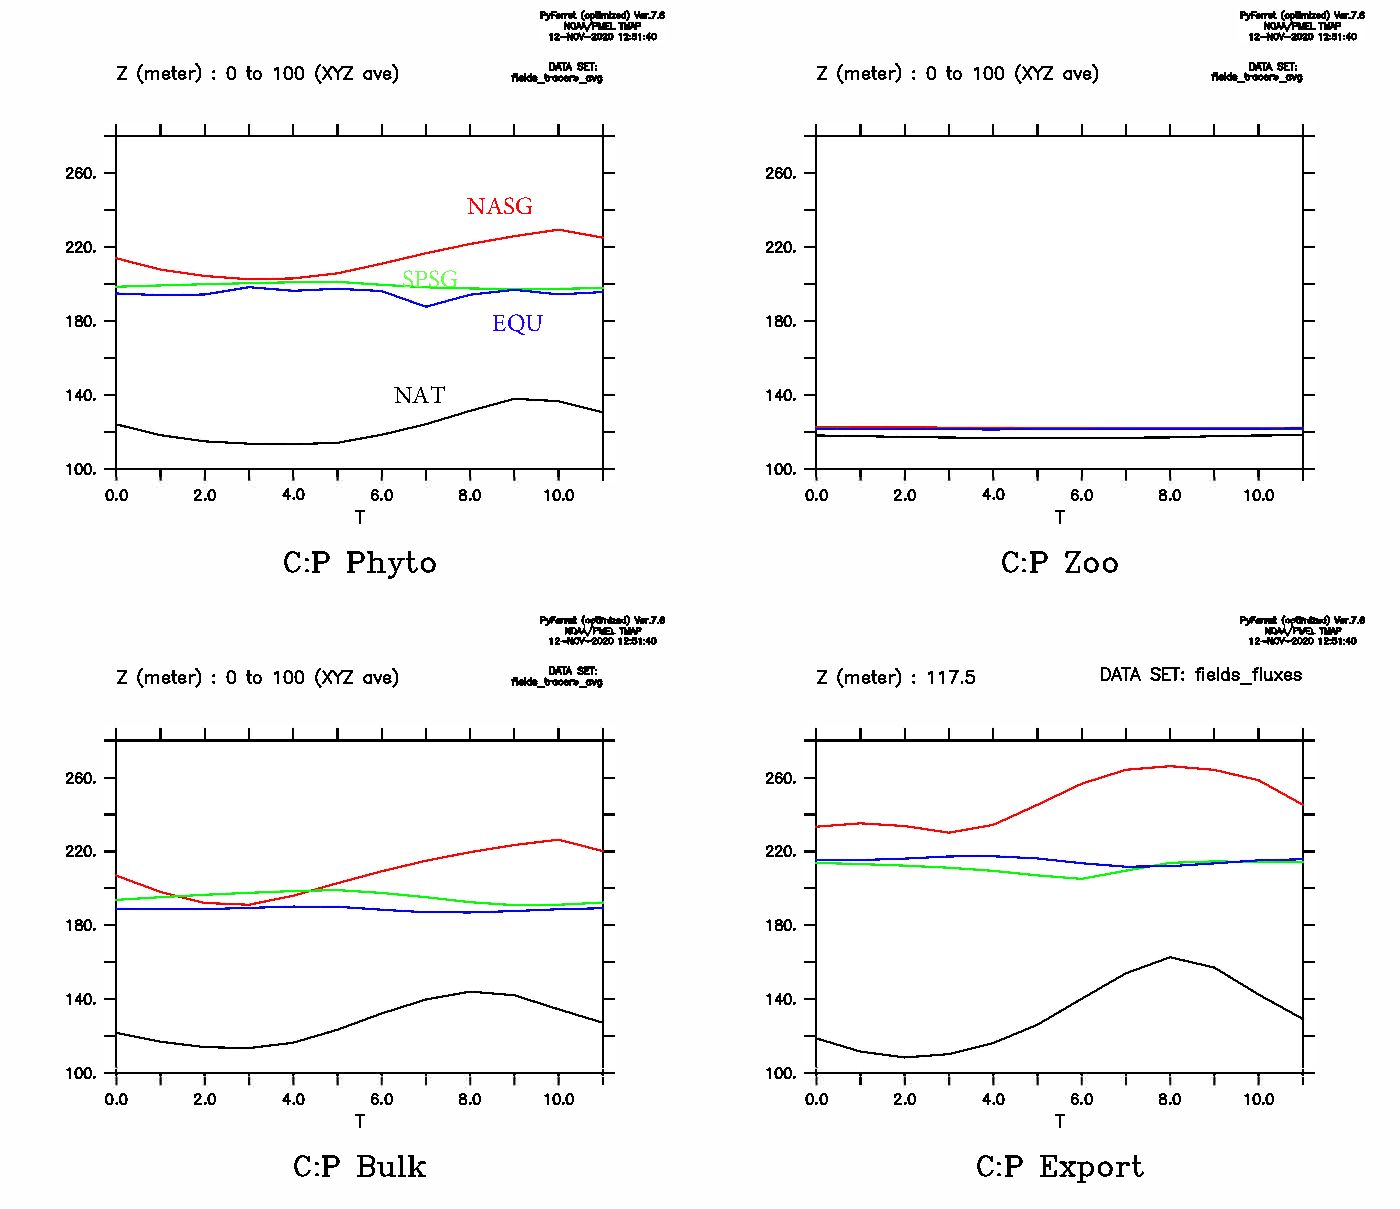
\includegraphics[scale=0.6]{cp_comparison.pdf}
   \caption[]{Modeled seasonal C:P of (a) Phytoplankton, (b) Zooplankton, (c) Bulk POM (= Detritus + Phytoplankton + Zooplankton), and (d) Export ratio at 100 m}
   \label{fig:cp_timeseries}
\end{figure}

Figure \ref{fig:cp_timeseries} shows the seasonal cycle of C:P. Phytoplankton C:P at NAT and NASG peaks in fall ($\sim$September) and is lowest during spring. This pattern generally follows that of SST and PO4, where low PO4/high SST leads to higher C:P. Seasonal variability of phytoplankton C:P at SPSG and EQU are smaller as the change in SST and nutrients are small. C:P of zooplankton remains around 117 even in gyres. As phytoplankton biomass is greater than that of zooplankton, C:P of bulk POM is similar in magnitude to that of phytoplankton. What's interesting is that C:P export is greater than C:P of phytoplankton and bulk POM at NASG, SPSG, and EQU. This is because excess carbon that is excreted by zooplankton is added to detrital POC pool leading to higher C:P of exported organic mater. At NAT, the different is relatively smaller because the stoichioemtric mismatch between phytoplankton C:P and zooplankton C:P is small. 

\item (Optional) We can also calculate export of DOC and DOP. The  code for making figrues is in my directory \verb|~/../tanio003/TMM2/Runs/MOPS/Testruns_ECCO/201108b/analyze_dom_export.jnl|.

\begin{figure}[h!]   % Insert Figure 8 here
   \centering
   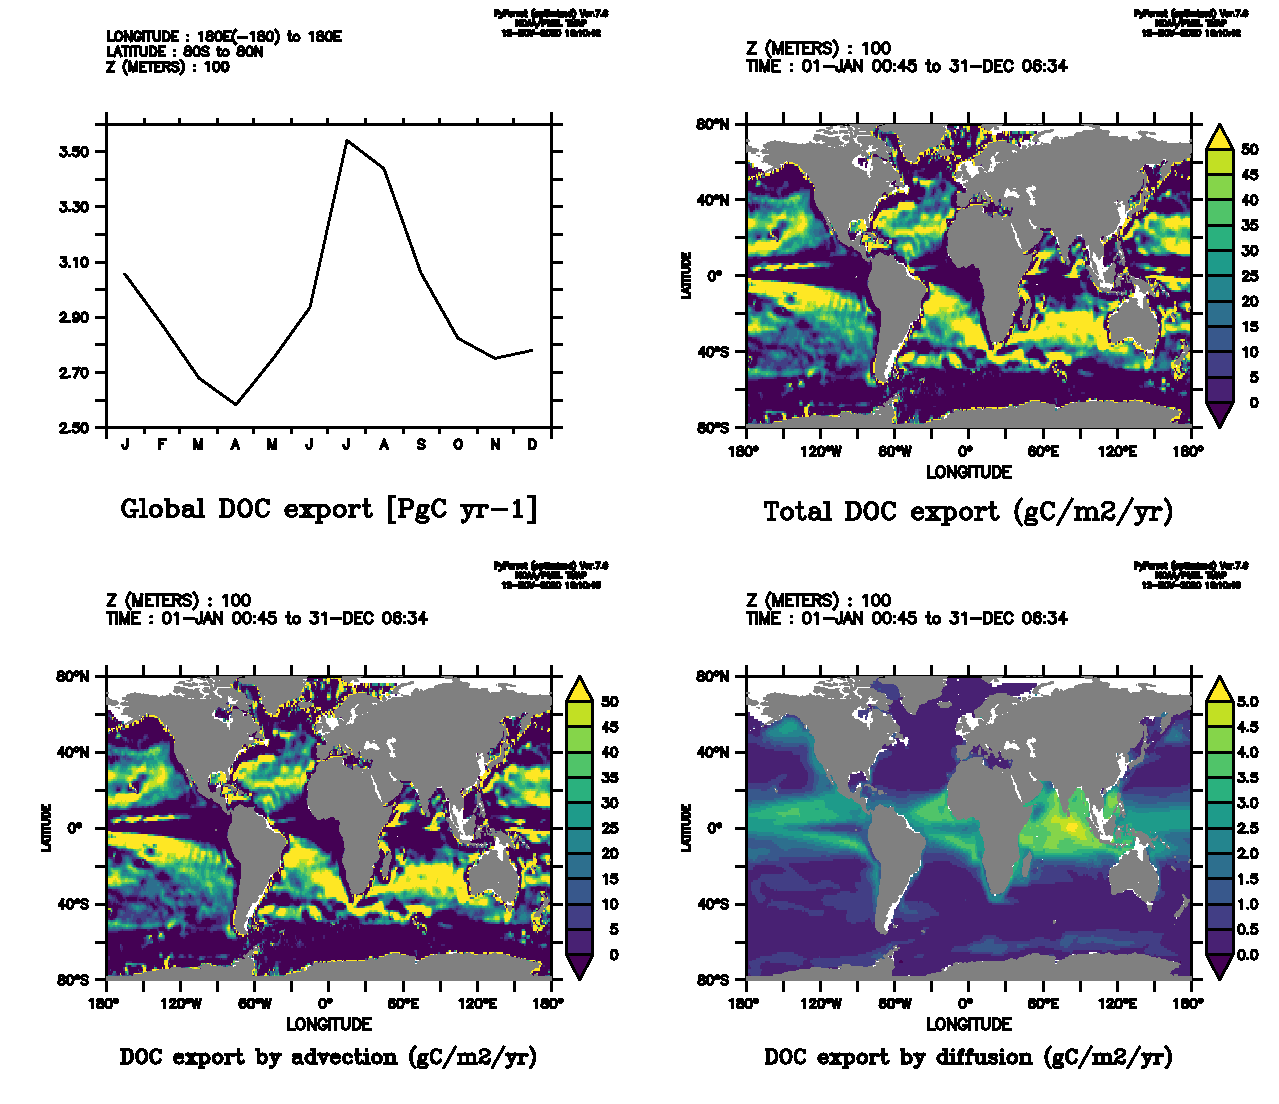
\includegraphics[scale=0.6]{doc_global.pdf}
   \caption[]{Modeled DOC export. (a) Monthly global DOC export at 100 m (b) Annual mean global DOC export (c) Annual mean global DOC export by advection, and (d) Annual mean global DOC export by diffusion.}
   \label{fig:doc_global}
\end{figure}

Figure \ref{fig:doc_global} shows that the total DOC export is around 3.0 PgC/yr which is factor of 2 greater than the previous modeling studies. This is mainly due to the fact that the DOC surface concentration at the moment is too high. This is something that need to be worked on. Majority of export occurs in the subtropical gyres by advection. Export due to diapycnal diffusion occurs in equatorial upwelling regions but the maginude is utmost 10$\%$

\begin{figure}[h!]   % Insert Figure 9 here
   \centering
   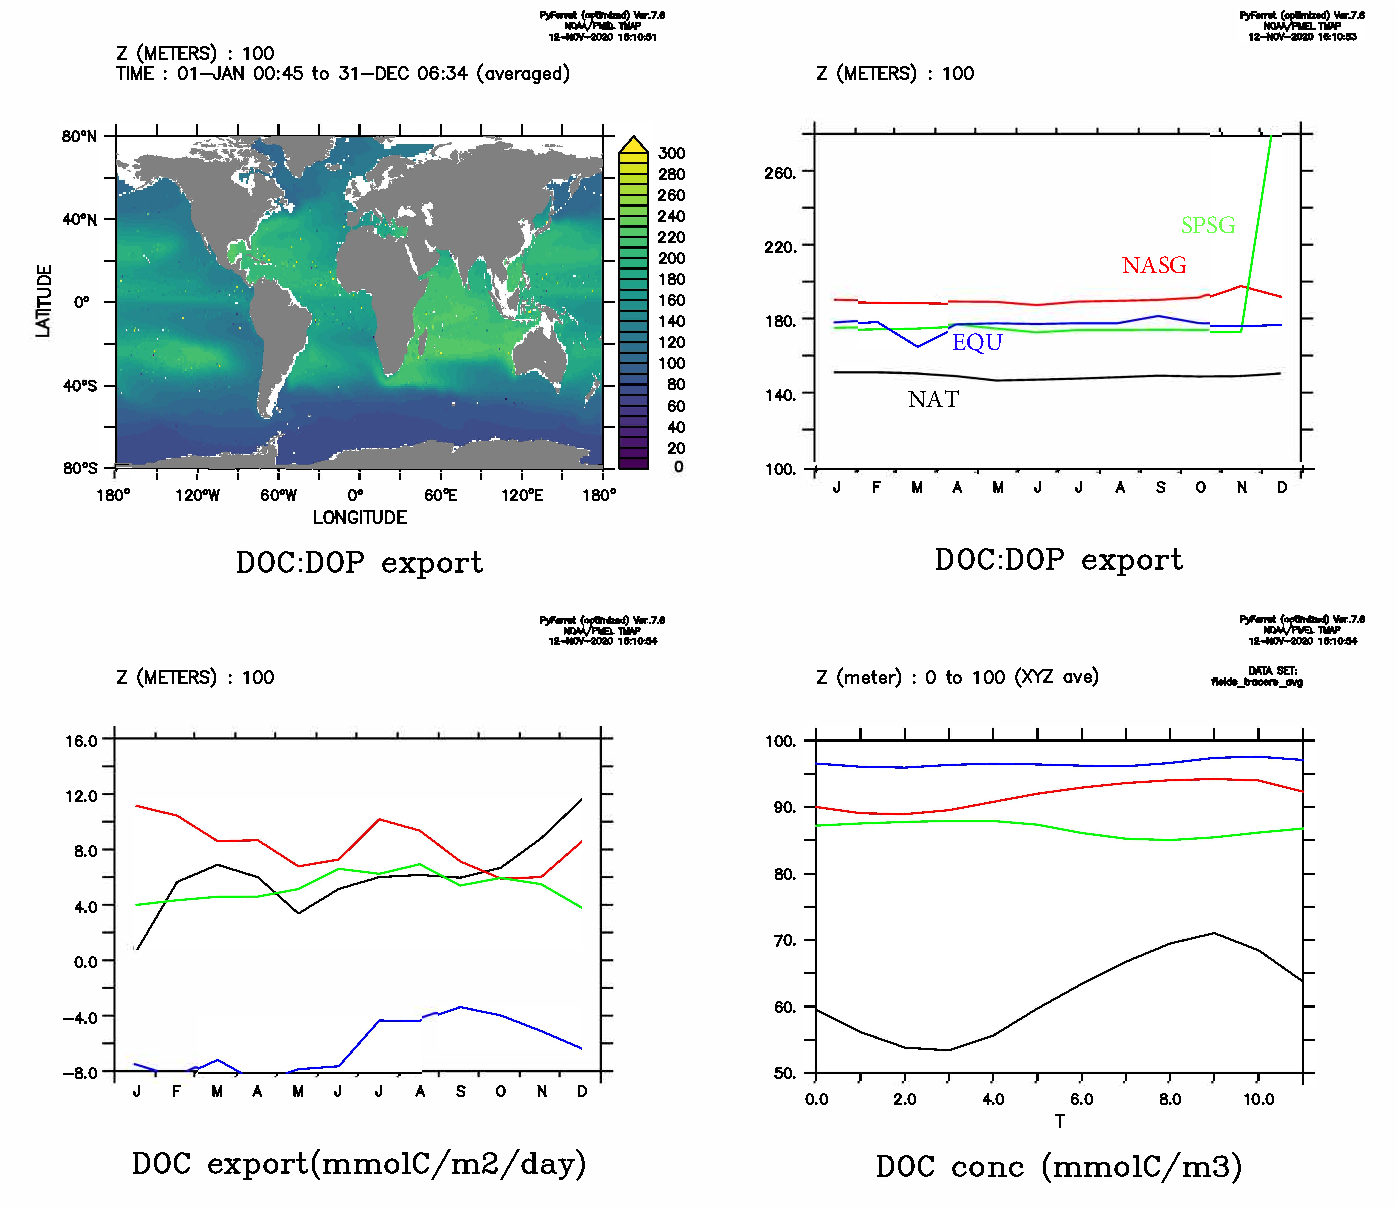
\includegraphics[scale=0.6]{doc_regional.pdf}
   \caption[]{Modeled DOC:DOP and regional DOC export. (a) Annual mean DOC:DOP export ratio at 100 m, (b) Annual mean DOC:DOP at 4 different regions, (c) Annual mean DOC export, and (d) Annual mean surface DOC concentration.}
   \label{fig:doc_regional}
\end{figure}

The seasonal pattern of DOC:DOP export in Figure \ref{fig:doc_regional} is similar to that of POC:POP export. Compared to POC:POP export (Fig. \ref{fig:cp_timeseries}(d)), temporal shift in DOC:DOP export is smaller. Another interesting thing is that DOC concentration (Fig. \ref{fig:doc_regional}(d)) and DOC export (Fig. \ref{fig:doc_regional}(c)) are not correlated in a predictable way. This shows the DOC export is much more nuanced as a result of interaction between physics (flow field) and biogeochemistry. DOC dynamics is something that has to be explored in more detail.

\end{enumerate}


\subsection{Study 3: Using MOBI+UVic to simulate isotope dynamics} 

For this study, we will explore ocean biogeochemical dynamics using the second version of MOBI (Model of Ocean Biogeochemistry and Isotopes). MOBI includes:
\begin{itemize}
\item \ce{NO3}, \ce{PO4}, and DFe as interactive nutrients.
\item 3 Phytoplankton classes (diazotrophs, coccolithophores, and other phytoplankton).
\item Zooplankton.
\item Detritus (dead POM).
\item \ce{CaCO3} is a prognostic variable and its production is calculated as a fraction of the detrirus produced by coccolithophores and zooplankton and it is sinking into the deep ocean where it dissolves.
\item Nitrogen (\ce{^15N}) and carbon (\ce{^13C}) isotopes are included in all compartments.
\item Radiocarbon (\ce{^14C}) is included only in the DIC compartment.
\item Dissolved \ce{O2} controls the water column denitrification. Benthic denitrification is calculated considerting subgridscale bathymetry.
\item DOM is calculated separately for C, N, and P (DOC, DON, DOP).
\item The most complex configuration has a total of 30 prognostic tracers.
\end{itemize}
\noin To learn different configurations of MOBI, refer to the primer by A. Schmittner (\url{https://github.com/tanio003/tmm/blob/TT_Release/Tutorial_MSI/MOBI2.0_Schmittner.pdf}). 

\textbf{In this exercise, we will try conducting a spin-up run for 1000 yrs using 28 prognostic tracers. Instructions will mostly follow that of S. Khatiwala.} MOBI is coupled to the UVicgit p model which consists of ocean general circulation at coarse resolution (1.8\times3.6 degrees, 19 vertical levels), a one-layer energy moisture balance atmaospheric component, a dynamic/thermodynamic sea ice model, and a land surface/dynamic vegetation module. 

\begin{enumerate}

\item Download the compatible versions of UVic ESCM 2.9 in the first level of your TMM directory
\begin{lstlisting}[style=DOS]
 $ cd ~/TMM2
 $ git clone https://github.com/tanio003/UVic2.9
\end{lstlisting}

\item Download the TMM called \verb|UVicOSUpicdefault|. To copy TMM in the shared directory, 
\begin{lstlisting}[style=DOS]
 $ cp -r ~/../shared/tmm/UVicOSUpicdefault $HOME/TMM2/
\end{lstlisting}

\noin Currently, MOBI can only be coupled to this TMM configuration (\verb|UVicOSUpicdefault|) because other TMMs like MITgcm models do not have bathymetry profile and hydrothermal Fe input masks.

\item Make a Run directory for TMM-MOBI. For this run, I call it \verb|Runs/MOBI/Test_spinup|. Copy \\ \verb|mobi2.0/src/Makefile| and \verb|mobi2.0/src/MOBI_TMM_OPTIONS.h| to this directory. 
\begin{lstlisting}[style=DOS]
 $ cd ~/TMM2
 $ mkdir -p Runs/MOBI/Test_spinup
 $ cd Runs/MOBI/Test_spinup
 $ cp -p $TMMROOT/models/current/mobi2.0/src/Makefile .
 $ cp -p $TMMROOT/models/current/mobi2.0/src/MOBI_TMM_OPTIONS.h . 
\end{lstlisting}
\noin Also, following the instructions at the top of Makefile, set the environmental variable \verb|$UVICESCMROOT| to point to the top level of the UVic ESCM 2.9. Add this to your \verb|.bashrc| for your future convenience.
\begin{lstlisting}[style=DOS]
 $ export UVICESCMROOT=$HOME/TMM2/UVic2.9
 echo $UVICESCMROOT
 /home/.../TMM2/UVic2.9
\end{lstlisting}

\item Copy the contents (including the subdirectories) of \verb|mobi2.0/matlab| and  \verb|mobi2.0/runscripts| to the test directory.
\lstset{emph={runscript,runscript_msi}, emphstyle=\color{green},emph={[2]InitialConditionProfiles}, emphstyle={[2]\color{blue}}}
\begin{lstlisting}[style=DOS]
 $ cp -p -R $TMMROOT/models/current/mobi2.0/matlab/* .
 $ cp -p $TMMROOT/models/current/mobi2.0/runscripts/* .
 $ ls
 control.in                Makefile
 get_mobi_diagnostic.m     make_input_files_for_mobi_model.m
 InitialConditionProfiles  make_input_files_for_mobi_model_write_ic.m
 load_diagnostics.m        MOBI_TMM_OPTIONS.h
 load_output.m             MOBI_tracer_names.txt
 load_output_sed.m         runscript
 load_output_time_avg.m    runscript_msi
\end{lstlisting}
\lstset{emph={}, emphstyle=\color{green},emph={[2]}, emphstyle={[2]\color{blue}}} % reset coloring

\item Edit the C preprocessor options in \verb|MOBI_TMM_OPTION.h| as necessary. In particular, you have to define the directive \verb|O_co2_user| (i.e., by \verb|# define O_co2_ccn_user|). See Appendix \ref{subsection:mobi_options} for what each of these options mean. 

\item Build the model with:
\begin{lstlisting}[style=DOS]
 $ make cleanall
 $ make tmmmobi
\end{lstlisting}
\noin If compiled properly, you would see an executable file \verb|tmmmobi| created along with a bunch of objective .o files. Don't worry about various warnings as long as they are not fatal. 

\item Generate the names tracers being simulated (as per the options set in \verb|MOBI_TMM_OPTIONS.h|) and their initial consitions. To do this, first set at the top of \verb|make_input_files_for_mobi_model_write_ic.m|. 
\lstset{language=matlab} 
\begin{lstlisting}[frame=single,basicstyle=\scriptsize,commentstyle=\color{blue}]
 % make_input_files_for_mobi_model_write_ic.m
  1 % Set toplevel path to GCMs configuration
  2 % base_path='/data2/spk/UVic_OSU_Matrix/LGM_WindPerturbation_Experiments/no_embm_awind2/picdefault';
  3 % base_path='/data2/spk/TransportMatrixConfigs/MITgcm_2.8deg';
  4 % base_path='/data2/spk/TransportMatrixConfigs/MITgcm_ECCO';
  5 % base_path='/data2/spk/TransportMatrixConfigs/MITgcm_ECCO_v4';
  6 base_path='~/TMM2/UVicOSUpicdefault';
  7 addpath(genpath('~/TMM2/tmm_matlab_code'));
 
\end{lstlisting}
\noin Then execute in MATLAB.
\begin{lstlisting}[style=DOS]
 >> make_input_files_for_mobi_model_write_ic
\end{lstlisting}

\item Compile and execute \verb|tmmmobiwrite|. 
\begin{lstlisting}[style=DOS]
 $ make tmmmobiwrite
 $ ./tmmmobiwrite
\end{lstlisting}
\noin This will write out \verb|MOBI_tracer_names.txt| containing the tracer names, and a corresponding set of *.dat text files (e.g., dic.dat) containing the vertical profile of tracer concentration. These names and initial profiles are used by \verb|make_input_files_for_mobi_model.m| to generate initial condition files (e.g., dicini.petsc). 

28 tracers created are:
\begin{enumerate}[label=(\arabic*)]
	\item \verb|imobipo4| = \ce{PO4} $[\mathrm{mmolP \ m^{-3}]}$
	\item \verb|imobiphyt| = Phytoplankton biomass $[\mathrm{mmolN \ m^{-3}]}$
	\item \verb|imobizoop| = Zooplankton biomass $[\mathrm{mmolN \ m^{-3}]}$
	\item \verb|imobidetr| = Detritus $[\mathrm{mmolN \ m^{-3}]}$
	\item \verb|imobidic| = DIC $[\mathrm{mmol \ m^{-3}]}$	
	\item \verb|imobidic13| = \ce{DI^{13}C} $[\mathrm{mmol \ m^{-3}]}$	
	\item \verb|imobiphytc13| = \ce{^13C} of Phytoplankton $[\mathrm{mmol \ m^{-3}]}$	
	\item \verb|imobizoopc13| = \ce{^13C} of Zooplankton $[\mathrm{mmol \ m^{-3}]}$	
	\item \verb|imobidetrc13| = \ce{^13C} of Detritus $[\mathrm{mmol \ m^{-3}]}$	
	\item \verb|imobidoc13| = \ce{DO^13C} $[\mathrm{mmol \ m^{-3}]}$	
	\item \verb|imobidiazc13| = \ce{^13C} of Diazotrophs $[\mathrm{mmol \ m^{-3}]}$		
	\item \verb|imobicoccc13| = \ce{^13C} of Coccolithophores $[\mathrm{mmol \ m^{-3}]}$	
	\item \verb|imobicaco3c13| = \ce{Ca^13CO_3} $[\mathrm{mmol \ m^{-3}]}$	
	\item \verb|imobidop| = \ce{DOP} $[\mathrm{mmolP \ m^{-3}]}$
	\item \verb|imobino3| = \ce{NO3} $[\mathrm{mmolN \ m^{-3}]}$
	\item \verb|imobidon| = \ce{DON} $[\mathrm{mmolN \ m^{-3}]}$	
	\item \verb|imobidiaz| = Diazotroph biomass $[\mathrm{mmolN \ m^{-3}]}$
	\item \verb|imobidin15| = \ce{DI^15N} $[\mathrm{mmol \ m^{-3}]}$	
	\item \verb|imobidon15| = \ce{DO^15N} $[\mathrm{mmol \ m^{-3}]}$	
	\item \verb|imobiphytn15| = \ce{^15N} of Phytoplankton $[\mathrm{mmol \ m^{-3}]}$	
	\item \verb|imobizoopn15| = \ce{^15N} of Zooplankton $[\mathrm{mmol \ m^{-3}]}$	
	\item \verb|imobidetrn15| = \ce{^15N} of Detritus $[\mathrm{mmol \ m^{-3}]}$		
	\item \verb|imobidiazn15| = \ce{^15N} of Diazotrophs $[\mathrm{mmol \ m^{-3}]}$	
	\item \verb|imobicoccn15| = \ce{^15N} of Coccolithophores $[\mathrm{mmol \ m^{-3}]}$	
	\item \verb|imobicocc| = Coccolithophores biomass $[\mathrm{mmolN \ m^{-3}]}$
	\item \verb|imobicaco3| = Calcium carbonate $[\mathrm{mmol \ m^{-3}]}$
	\item \verb|imobidfe| = Dissolved iron $[\mathrm{nmol \ m^{-3}]}$
	\item \verb|imobidetrfe| = Detrital iron $[\mathrm{nmol \ m^{-3}]}$
\end{enumerate}

\item Make a directory \verb|InitialConditionProfiles| and copy the *.dat files into it. By default \\ \verb|make_input_files_for_mobi_model.m| (mentioned later) will look in this directory for the *.dat files.
\begin{lstlisting}[style=DOS]
 $ cp -p *.dat InitialConditionProfiles/
\end{lstlisting}

\noin (Note-1): There are already copies of \verb|MOBI_tracer_names.txt| and \verb|InitialConditionProfiles/| in matlab/ but S.Khawtiwala recommends you still go through this step to generate tracer names consistent with your version of \verb|UVic/MOBI| and \verb|MOBI_TMM_OPTIONS.h|.

\noin (Note-2): The order of tracers in \verb|MOBI_tracer_names.txt| is the same as that in which you specify initial condition, output and time average files in the TMM-MOBI run script. You can reduce the tedium (and chances of making a mistake) of generating the correct sequence to specify in the run script by executing this on the command line: 
\begin{lstlisting}[style=DOS]
 $ printf "%sini.petsc," `tr '\n' ' ' < MOBI_tracer_names.txt` | sed 's/,*$//g'
\end{lstlisting}
(The tr replaces newlines with spaces to put all tracer names on a single line, 
the printf appends "ini.petsc," to each tracer name, and the sed strips out the 
final comma.)

\noin (Note-3): \verb|tmmmobiwrite| uses UVic routines where initial condition profiles are set. The code for this is hardwired for the standard UVic grid with 19 levels. If you're using TMs from a different ocean model you will need to modify \verb|make_input_files_for_mobi_model.m| accordingly to specify initial conditions corresponding to your grid. You will also need to change the number of levels (in kilometers) in \verb|size.h|.

\item Set the path at the top of \verb|make_input_files_for_mobi_model.m| and execute in MATLAB. Make sure to set the correct timestep of 28800 seconds. 
\lstset{language=matlab} 
\begin{lstlisting}[frame=single,basicstyle=\scriptsize,commentstyle=\color{blue}]
 % make_input_files_for_mobi_model.m
  1 % Set toplevel path to GCMs configuration
  2 % base_path='/data2/spk/UVic_OSU_Matrix/LGM_WindPerturbation_Experiments/no_embm_awind2/picdefault';
  3 % base_path='/data2/spk/TransportMatrixConfigs/MITgcm_2.8deg';
  4 % base_path='/data2/spk/TransportMatrixConfigs/MITgcm_ECCO';
  5 % base_path='/data2/spk/TransportMatrixConfigs/MITgcm_ECCO_v4';
  6 base_path='~/TMM2/UVicOSUpicdefault';
  7 addpath(genpath('~/TMM2/tmm_matlab_code'));
  8
  9 periodicForcing=1
 10 periodicMatrix=1
 11
 12 dt=28800; % time step to use
 ....
\end{lstlisting}
\begin{lstlisting}[style=DOS]
 >> make_input_files_for_mobi_model
\end{lstlisting}

\item Edit the namelists in \verb|control.in| as necessary. The important variables you 
must set are:

\begin{itemize}
\item \verb|dtts| in the \verb|&tsteps| namelist: this MUST match the time step argument to the run time option called \verb|-biogeochem_deltat| in the runscript. This sets the tracer advection-diffusion timestep (28800 [seconds] for UVIc model). 
\item \verb|co2ccn| and \verb|dc14ccn| in the \verb|&carbon| namelist. 
\item \verb|dtnpzd| in the \verb|&npzd| namelist. Set this so that \verb|dtts| is a multiple of \verb|dtnpzd|. For stability, \verb|dtnpzd| (in seconds) should not exceed 1/3\textsuperscript{rd} of a day (in seconds). The default is \verb|dtpnzd|=14400 = 1/2 of ocean timestep. 
\end{itemize}
\noin See Appendix \ref{subsection:mobi_params} for what each of these other options mean in \verb|control.in|. 

\item Edit runscript as necessary. Also see (NOTE-2 in \verb|#|9). It takes about 8 hours to complete 1000 yr run with 2 nodes (48 cores). In this run, we will output monthly tracer averages as well as diagnostic fluxes in the final year of the run. Tracer snapshot concentrations will be outputted every 100 years.

\lstset{language=sh} 
\begin{lstlisting}[frame=single,basicstyle=\scriptsize,commentstyle=\color{blue}]
 # runscript_msi
\end{lstlisting}
\noin (NOTE-1): If turning on sediments and running on a smaller number of CPUs you should unlimit stacksize. Otherwise you may get a segmentation fault. Don't worry about this too much for MSI users but you can check just in case by:
\begin{lstlisting}[style=DOS]
 $ ulimit -H -a
 ...
 stack size              (kbytes, -s) unlimited
\end{lstlisting}

\item Submit your job to MSI queue.
\begin{lstlisting}[style=DOS]
 $ sbatch runscript_msi
\end{lstlisting}

\item Whilte you wait for the run to be completed, set the path at the top of the load*.m scripts to read in the output in Matlab. To make all the output netcdf files in matlab at once, run \verb|process_output.m|. For this exercise, the sedimentary module, hence the sedimentary output is suppressed. 

\noin Each .nc file is spewed out one by one. There are different kinds of output files that are being produced:
\begin{itemize}
 \item F\_**.nc (e.g., F\_dic.nc): Surface Downward Fluxes [mol $\mathrm{m^{-2} s^{-1}}$]. Edit "available\_diagnostics.txt" to select which fluxes to create.
 \item O\_**.nc (e.g., O\_phytnpp.nc): Various biogeochemical fluxes and concentrations that are calculated in the model. Units are in [mol $\mathrm{m^{-2} s^{-1}}$] or [mol $\mathrm{m^{-2}}$]. Edit "available\_diagnostics.txt" to select which fluxes to create.
 \item **.nc (e.g., PO4.nc): Snapshot concentrations of tracers. Edit "MOBI\_tracer\_names.txt" to select which tracers you want to convert to .nc files.
 \item **mmavg.nc (e.g., PO4mmavg.nc): Time-averaged concetrations of tracers. Edit "MOBI\_tracer\_names.txt" to select which tracers you want to convert to .nc files.
\end{itemize}

\item Display outputs. Here, we will make figures for \Delta\ce{^14C} [permil] and \delta\ce{^13C} [permil] at the final year of the run and compare with observations. The code for making the following two figures is my directory \verb|~/../tanio003/TMM2/Runs/MOBI/Test_spinup/analyze_mobi_spinup.jnl|.

\begin{figure}[h!]   % Insert Figure 10 here
   \centering
   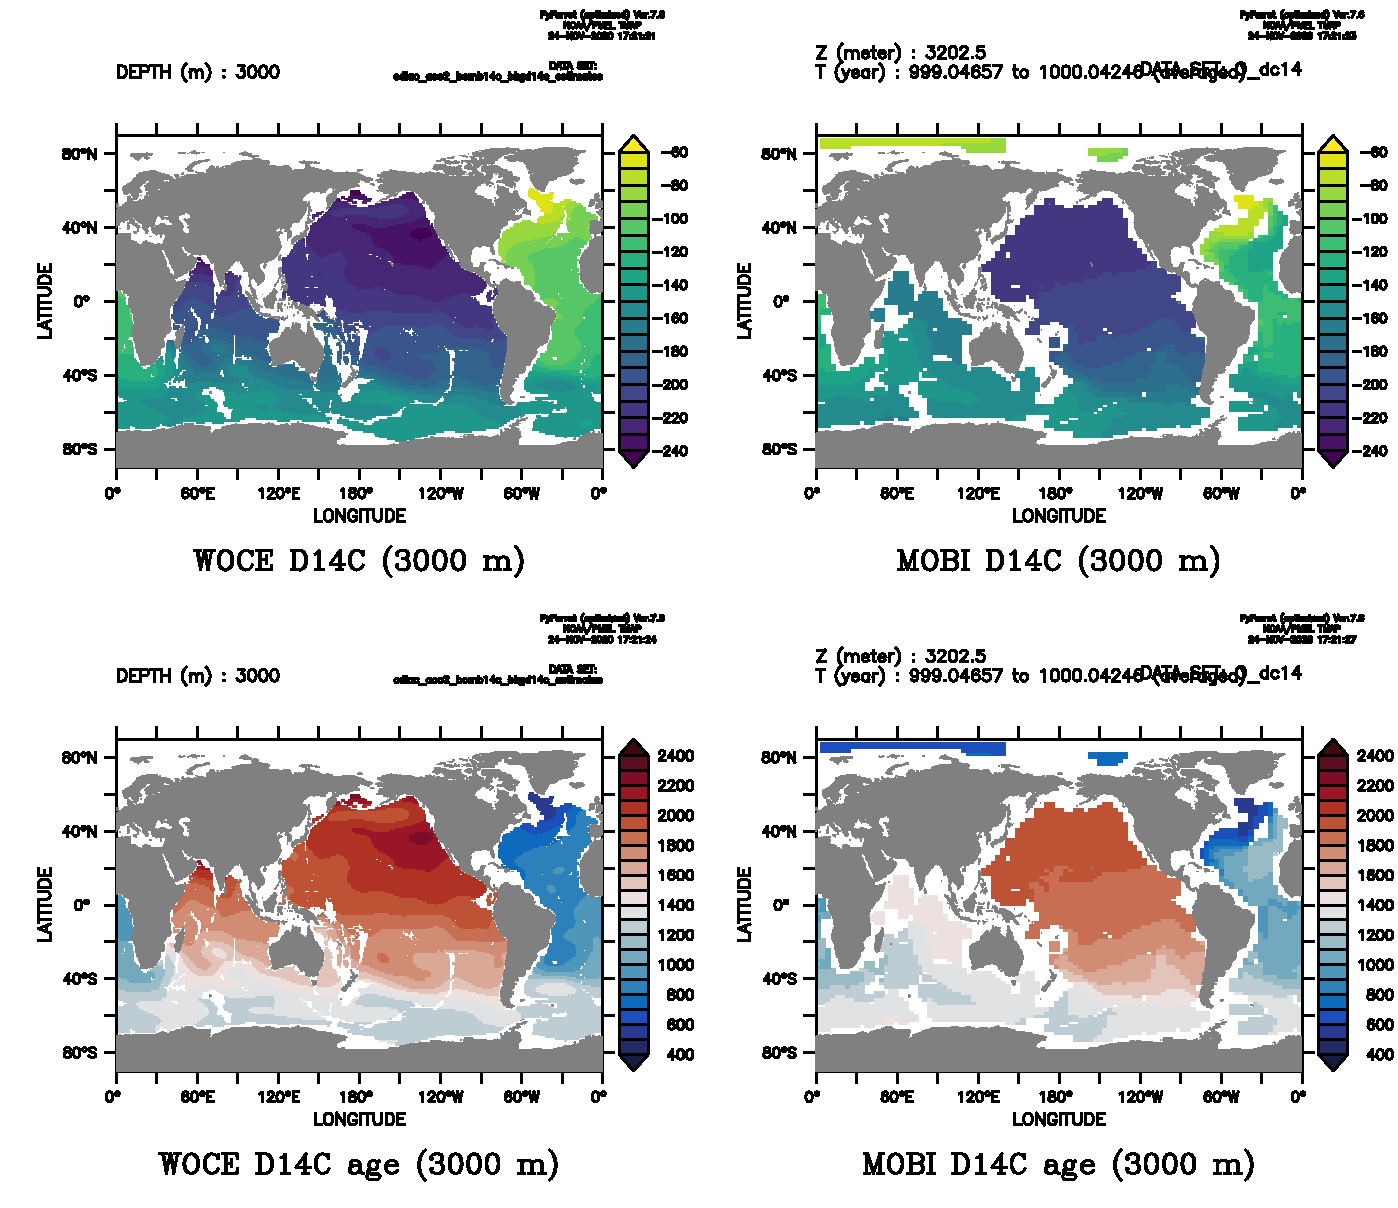
\includegraphics[scale=0.5]{MOBI_WOCE_C14.pdf}
   \caption[]{Observed and modeled natural \Delta\ce{^14C} and \ce{^14C} age at 3000 m. (a) Data-derived estimtate of \Delta\ce{^14C} from WOCE \citep{Key04} at 3000 m (b) Modeled  \Delta\ce{^14C} by MOBI at Year 1000 (c) Observed \ce{^14C} age at 3000 m, and (d) Modeled \ce{^14C} age at 3000 m.}
   \label{fig:c14_mobi}
\end{figure}

Figure \ref{fig:c14_mobi} compares observed and modeled radiocarbon ages. Although \ce{^14C} has not fully reached steady-state after 1000 yrs (figure not shown), the MOBI seems to reproduce the observed pattern of deep-sea natural radiocarbon age quite well. 

\begin{figure}[h!]   % Insert Figure 11 here
   \centering
   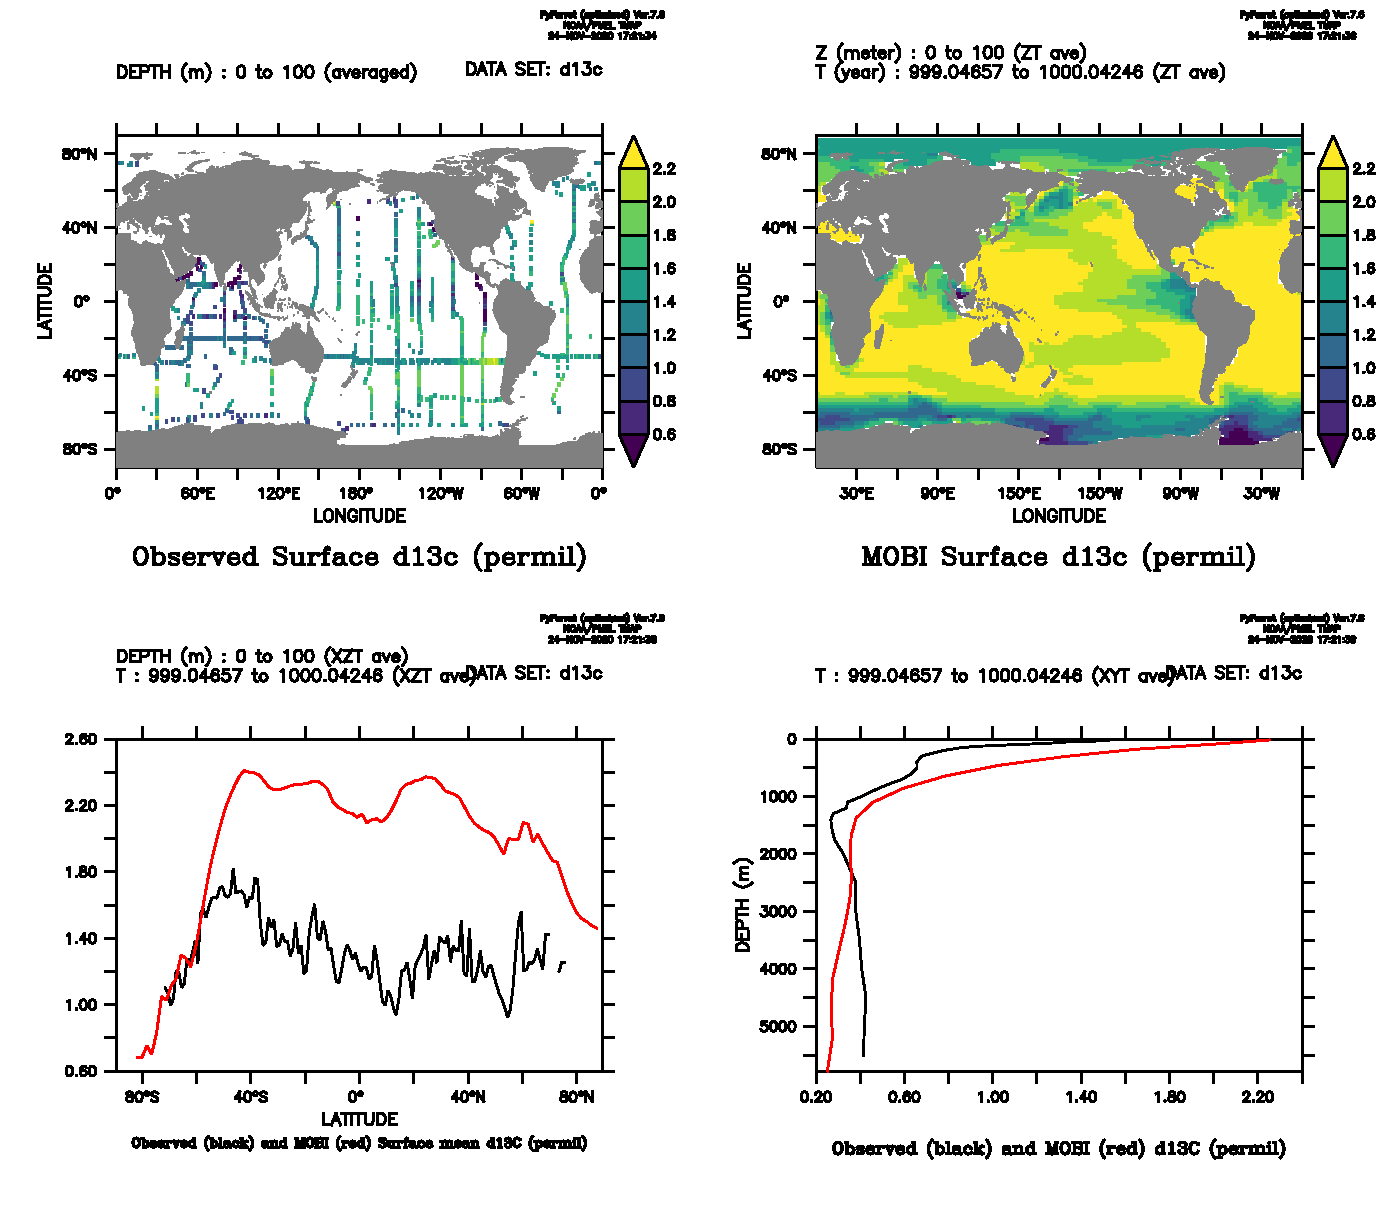
\includegraphics[scale=0.5]{MOBI_OBS_C13.pdf}
   \caption[]{Observed and modeled \delta\ce{^13C} at the surface and the depth profile. (a) Observed \delta\ce{^13C} of DIC at 0-100 m from years 1990 to 2005 \citep{Schmittner13}  (b) Modeled surface \delta\ce{^13C} by MOBI at Year 1000 (c) Observed (black) and Modeled (red) zonal average surface \delta\ce{^13C} (d) Global mean depth-profile of observed (black) and modeled (red) \delta\ce{^13C}.}
   \label{fig:c13_mobi}
\end{figure}

Figure \ref{fig:c13_mobi} compares observed and modeled \delta\ce{^13C}. In general, modeleded \delta\ce{^13C} overestimates the observed value in the surface ocean, but it captures the large-scale pattern. Biological fractionation and the sinking of isotopically light \delta\ce{^13C} organic matter from the surface into the interior ocean leads to low \delta\ce{^13C} DIC values at depths and in high latitude surface waters and high values in the upper ocean at low latitudes with maxima in the subtropics. Below 1000 m, model reproduces the observed pattern fairly well.

\end{enumerate}

%%%%%%%%%%%%%%%
\subsection{Study 4: Using Transport Matrix to Caluclate Steady State Model Circulation Age}
Here, we will breifly go over how to calculate steady state model circulation age anf radiocarbon distributions. For full mathematical details, refer to \citet{Khatiwala05} and  \citet{Khatiwala07}. 

In TMM, tracer vector \textbf{c} at timestep \textit{n+1} can be calculated from the concentration and the transport matrix \textbf{A} at time step \textit{n}:
\begin{equation}
   \mathbf{c}^{n+1}= \mathbf{A}_i^{n}(\mathbf{A}_e^{n}\mathbf{c}^{n} + \mathbf{q}^n)   \label{eq:eq_tmm1}
\end{equation}
where $\mathbf{A}_e$ is the TM for the explicit-in-time component of advection-diffusion, and $\mathbf{A}_i$ the matrix for implicit transport. \textbf{q} represents the source and sinks. The TMs $\mathbf{A}_e$ and $\mathbf{A}_i$ are both extremely sparse. Physically, this is because of the finite speed of advection and diffusion (i.e., in a single timestep tracer can only communicate with their nearest neighbors). In the vertical, convection can spread the tracer further but this is restricted to small regions in high latitudes and is captured entirely by $\mathbf{A}_i$. 

In some cases, tracers are subject to a prescribed concentration (BC) at the surface. To solve such equations, we convert Equation (\ref{eq:eq_tmm1}) into an equation for the time evolution of the interior tracer field as follows:
\begin{equation}
   \mathbf{c}_I^{n+1}= \mathbf{A}_i^{I}(\mathbf{A}_e^{I}\mathbf{c}_I^{n} + \mathbf{B}_e\mathbf{c}_B^{n} + \mathbf{q}_I^n) + \mathbf{B}_i\mathbf{c}_B^{n+1}   \label{eq:eq_tmm2}
\end{equation}
where $\mathbf{c}_I$ is the vector of interior tracer concentrations, $\mathbf{c}_B$ the vector of prescribed, possibly time-dependent surface boundary values, and $\mathbf{q}_I$ the interior source/sink term. Notice that we split $\mathbf{A}_e$ into an ``interior'' matrix $\mathbf{A}_e^{I}$ and a ``boundary'' matrix $\mathbf{B}_e$. Implicit matrix $\mathbf{A}_i$ is split into an interior and a boundary component in the same manner. The square interor matrix describes the transport of tracer between interior grid points. The rectangular boundary matrix describes the exchange of tracer between the surface boundary points and the inteior.

In many cases, we are interested in the equilibrium solutions. Using Equations (\ref{eq:eq_tmm1}) and (\ref{eq:eq_tmm2}), we can directly compute stead-state distributions of tracers without the need for long transient integrations, for example if the source/sink and boundary terms are simple linear terms. Steady-state solutions can be analytically obtained by setting  $\mathbf{c} \equiv \mathbf{c}^{n+1}=\mathbf{c}^{n}$ in Equation (\ref{eq:eq_tmm1}) and solving for \textbf{c}. For an illustration, we will compute using this method: (1) the steady state ideal age (mean age), and (2) radiocarbon $\Delta^{14}\mathrm{C}$. 

\begin{enumerate}[label=(\arabic*)]
\item Ideal age $\boldsymbol{\tau}_m$: In a conventional GCM, calculation of mean age requires integrating a tracer with a unit source in the interior and a surface BC of zero concentration to steady state, an expensive computation even at coarse resolution. In our notation of Equation (\ref{eq:eq_tmm2}), $\mathbf{c}_B = \mathbf{0}$ and $\mathbf{q}_I = dt\mathbf{1}$, where \textbf{1} is a vector of 1's and \textit{dt} is the time step. In ECCO, \textit{dt} is 1/16 d = 5400 seconds, which is same as that of MOPS-ECCO. (In MIT2.8, I recommend using \textit{dt} of 1/2 d.). Substituting these in Equation (\ref{eq:eq_tmm2}), we get 
\begin{equation}
   (\mathbf{A}_i^{I}\mathbf{A}_e^{I}-\mathbf{I})\boldsymbol{\tau}_m = -dt\mathbf{A}_i^{I}\mathbf{1}   \label{eq:eq_tmm3}
\end{equation}
which can be readily solved for $\boldsymbol{\tau}_m$ by,
\begin{equation}
   \boldsymbol{\tau}_m = (\mathbf{A}_i^{I}\mathbf{A}_e^{I}-\mathbf{I})^{-1}(-dt\mathbf{A}_i^{I}\mathbf{1})   \label{eq:eq_tmm4}
\end{equation}

\begin{figure}[h!]   % Insert Figure 12 here
   \centering
   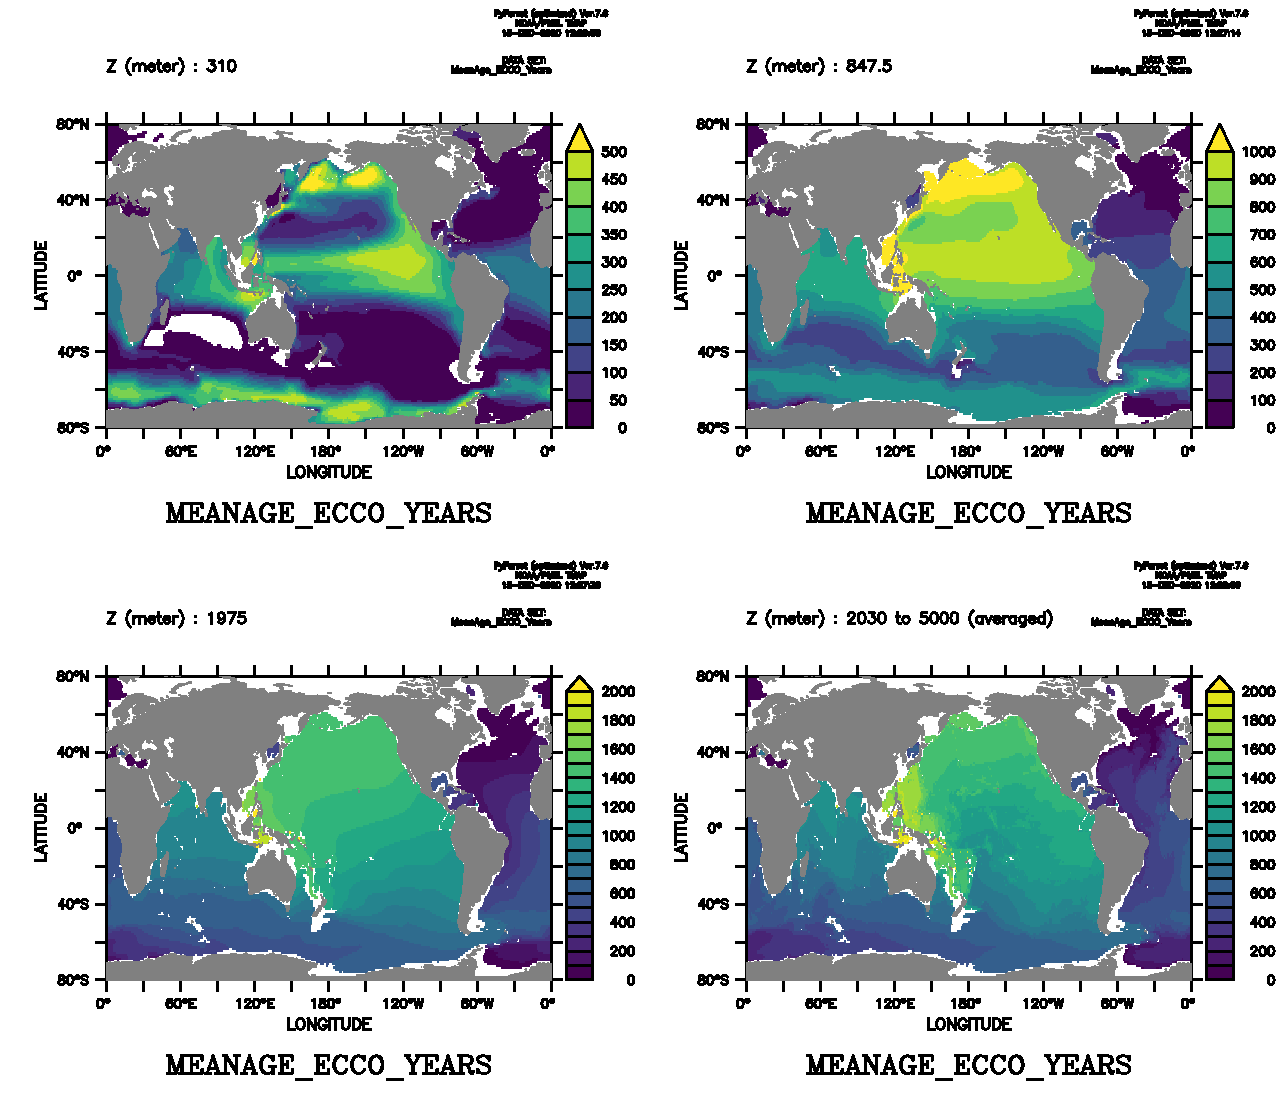
\includegraphics[scale=0.65]{meanage_ecco.pdf}
   \caption[]{Modeled annual mean circulation age (in years) for the ECCO model at 4 different depths.}
   \label{fig:meanage_ecco}
\end{figure}

Figure \ref{fig:meanage_ecco} shows the mean age at four different depths obtained with the annual mean TM for ECCO model. MATLAB codes used in calculating mean age are available in the directory \\ ``\verb|/home/matsumot/tanio003/TMM2/steady_state/ecco_meanage.m|''. To run this file, you need to use the shell script \verb|ecco_meanage.sh| in the same directory and takes 10 minutes or so on MSI. Note that I used the function \verb|calc_steadystate_tracer| in the directory ``\verb|~/TMM2/tmm_matlab_code/TMM|'' created by S. Khatiwala. See that file for more details on the syntax. 

\item Radiocarbon $\Delta^{14}\mathrm{C}$ [Method 1]: In the first method of calculating $\Delta^{14}\mathrm{C}$, we prescribe the surface value using the gridded GLODAP data by \cite{Key04} and compute steady state interior concentration. In our notation of Equation (\ref{eq:eq_tmm2}), $\mathbf{q}_I = -\lambda\mathbf{c}$, where \lambda \ is the decay constant for \ce{^14C} (half-lie of 5370 years) and $\mathbf{c}_B$ is the surface boundary concentration from GLODAP. Following \cite{Toggweiler89}, \textbf{c} is related to conventional $\Delta^{14}\mathrm{C}$ units by,
\begin{equation}
   \Delta^{14}\mathrm{C} \ (\mathrm{permil}) = (c - 100)\times 10   \label{eq:eq_tmm5}
\end{equation}
In other words, we compute \textbf{c} first then convert to  $\Delta^{14}\mathrm{C}$ via Equation (\ref{eq:eq_tmm5})).

We can write Equation (\ref{eq:eq_tmm2}) as, 
\begin{equation}
   (\mathbf{A}_i^{I}\mathbf{A}_e^{I}-\lambda\mathbf{A}_i^{I}-\mathbf{I})\mathbf{c} =-\mathbf{A}_i^{I}\mathbf{B}_e\mathbf{c}_B - \mathbf{B}_i\mathbf{c}_B = -\mathbf{A}_i^{I}(\mathbf{B}_e\mathbf{c}_B+(\mathbf{A}_i^{I})^{-1}\mathbf{B}_i\mathbf{c}_B)   \label{eq:eq_tmm6}
\end{equation}
The second term on the right hand side of the equation is collected by $\mathbf{A}_i^{I}$ for the later convenience. In the MATLAB code, the second terms needs to be divided by \textit{dt} because $\mathbf{B}_i\mathbf{c}_B$ is measured on the discrete time, while $\mathbf{B}_e\mathbf{c}_B$ is on the continuous time. We solve for \textbf{c} in Equation (\ref{eq:eq_tmm6}) by,
\begin{equation}
   \mathbf{c} = -(\mathbf{A}_i^{I}\mathbf{A}_e^{I}-\lambda\mathbf{A}_i^{I}-\mathbf{I})^{-1}\mathbf{A}_i^{I}(\mathbf{B}_e\mathbf{c}_B+(\mathbf{A}_i^{I})^{-1}\mathbf{B}_i\mathbf{c}_B)   \label{eq:eq_tmm7}
\end{equation}
then convert to $\Delta^{14}\mathrm{C}$ by Equation (\ref{eq:eq_tmm5}). 

\begin{figure}[h!]   % Insert Figure 13 here
   \centering
   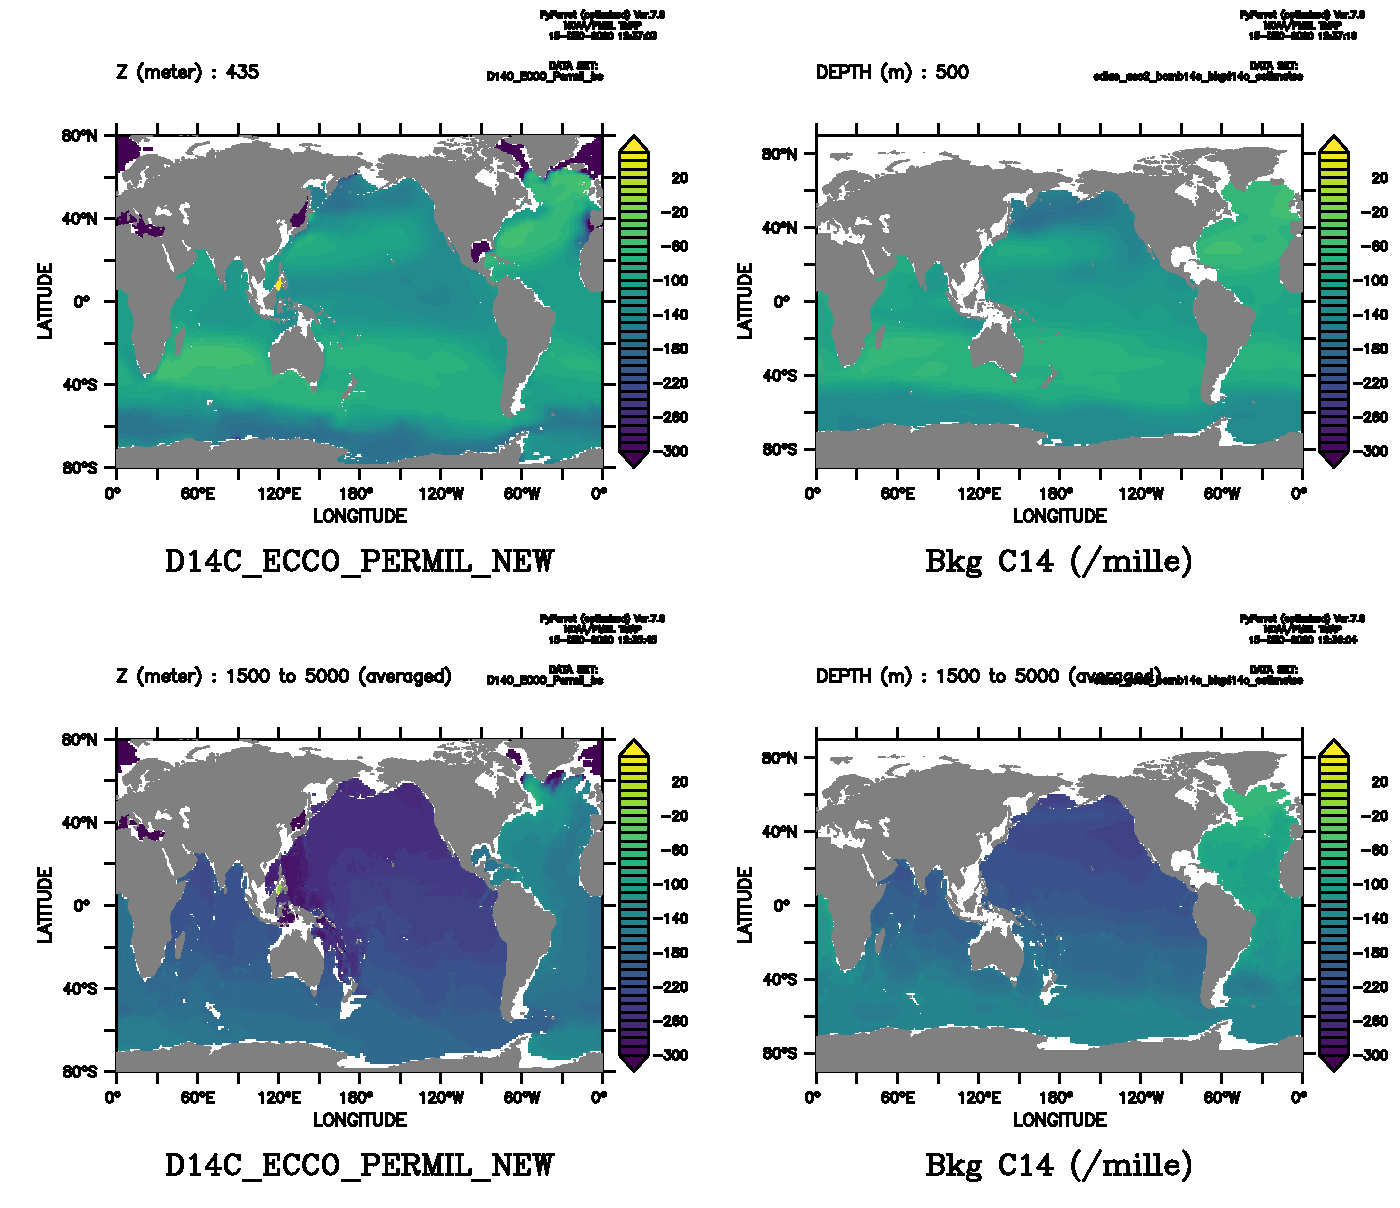
\includegraphics[scale=0.65]{D14C_ecco.pdf}
   \caption[]{Modeled (Left) and GLODAP-derived (right) natural annual mean $\Delta^{14}\mathrm{C}$ (in permil) at 2 different depths. Model used is ECCO and GLODAP map is from \cite{Key04}.}
   \label{fig:c14_ecco}
\end{figure}

Figure \ref{fig:c14_ecco} shows the modeled (left panel) and GLODAP-based $\Delta^{14}\mathrm{C}$ (right panel) at 500 m and at 1500-5000 m. We can see that modeled $\Delta^{14}\mathrm{C}$ does a good job in reproducing the observed radiocarbon pattern. In the deep ocean, modeled radiocarbon is slightly older than that of observation.  MATLAB codes used in calculating radiocarbon and its \ce{14C} age (figures not shown) are available in the directory \\ ``\verb|/home/matsumot/tanio003/TMM2/steady_state/ecco_radiocarbon_bc.m|''. To run this file, you need to use the shell script \verb|ecco_radiocarbon_bc.sh| in the same directory and takes 10 minutes or so on MSI. You would also need to copy the GLODAP surface boundary condition file ``\verb|bkgc14_cdiac_regird.mat|'' in the same directory, which is a surface backgroud radiocarbon concentration regridded to the ECCO grid.

\item Radiocarbon $\Delta^{14}\mathrm{C}$ [Method 2]: Alternatively, we can impose the surface boundary condition where $\Delta^{14}\mathrm{C}$ is restored to 0 ($\mathbf{c} = \mathbf{100} $) with a wind speed-dependent timescale, as done in \cite{Khatiwala05} and \cite{Khatiwala07}. In this case, we can write Equation (\ref{eq:eq_tmm1}) as, 
\begin{equation}
   \mathbf{c}^{n+1}= \mathbf{A}_i^{n}(\mathbf{A}_e^{n}\mathbf{c}^{n} -k(\mathbf{c}-\mathbf{100}) - \lambda\mathbf{c})   \label{eq:eq_tmm9}
\end{equation}
where \textit{k} is the wind speed depdendent timescale following Equation (11) of \cite{Toggweiler89}:
\begin{equation}
   k \ [\mathrm{days^{-1}}]= \frac{3.5\times(w-2) \ [\mathrm{mol\ m^{-2} \ yr^{-1}}]}{2.0 \ [\mathrm{mol\ m^{-3} }]\times DZ_1 \times 365 \ [\mathrm{days\ yr^{-1} }]  }\times 1.2   \label{eq:eq_tmm10}
\end{equation}
where \textit{w} is the spatially-variable wind speed in $\mathrm{m \ s^{-1}}$ and $DZ_1$ is the depth of the surface layer in meters (5 m in ECCO). Windspeed \ $w = 0$ when the grid box is completely covered by ice. Equation (\ref{eq:eq_tmm9}) can be rearranged and solved for \textbf{c} 
\begin{equation}
   \mathbf{c} = -(\mathbf{A}_i^{I}\mathbf{A}_e^{I}-\lambda\mathbf{A}_i^{I}- k\mathbf{A}_i^{I}- \mathbf{I})^{-1}\mathbf{A}_i^{I}(\mathbf{100}k)   \label{eq:eq_tmm11}
\end{equation}
There is a MATLAB script called in my directory \\ ``\verb|/home/matsumot/tanio003/TMM2/steady_state/ecco_radiocarbon.m|'' that computes $\Delta^{14}\mathrm{C}$ and age this way. The result is very similar to that of the first method (Figure not shown). All the netcdf files are in my output directory ``\verb|/home/matsumot/tanio003/TMM2/steady_state/output|''.
 
\end{enumerate}


%%%%%%%%%%%%%%%

%%%%%%%%%%%%%%%
\section{Appendix}

\subsection{Downloading PyFerret on MSI}

\begin{enumerate}
\item Install miniconda on your home directory. This is a free cross-platform for Python distribution from Continuum Analytics. 
\begin{lstlisting}[style=DOS]
 $ cd ~
 $ module purge
 $ wget https://repo.anaconda.com/miniconda/Miniconda3-latest-Linux-x86_64.sh
 $ bash Miniconda3-latest-Linux-x86_64.sh
\end{lstlisting}
\noin Follow the prompts on the installer screens. If you are unsure about any setting, accept the defaults. To make the changes take effect, close and then re-open your terminal window. Once installed you should find new directory called \verb|miniconda3| on your home directory.

\item Execute the following command to install \verb|pyferret| as well as \verb|ferret_datasets| (the default Ferret datasets) into conda.
\begin{lstlisting}[style=DOS]
 $ conda create -n PyFERRET -c conda-forge pyferret ferret_datasets --yes
\end{lstlisting}
\noin \verb|PyFERRET| is the environment name where \verb|pyferret| is installed. You can change that to any name you like.

\item To start using PyFerret, execute the following commands (replace \verb|PyFERRET| with whatever environment name you used):
\begin{lstlisting}[style=DOS]
(base) $ conda activate PyFerret
(PyFERRET) $ pyferret
  	NOAA/PMEL TMAP
 	PyFerret v7.6 (optimized)
 	Linux 4.15.0-1089-azure - 06/25/20
 	18-Sep-20 15:07

yes?
\end{lstlisting}

\item (Optional) You may with to add directories to \verb|FER_DATA| and \verb|FER_GO|:
\begin{lstlisting}[style=DOS]
(PyFERRET) $ export FER_DATA="$FER_DATA /my/path/to/big/data/dir"
(PyFERRET) $ export FER_GO="$FER_GO /my/path/to/custom/ferret/scripts"
\end{lstlisting}

\item Once you are done working with PyFerret you can leave this environment, if you wish, with the command:
\begin{lstlisting}[style=DOS]
(PyFERRET) $ conda deactivate
(base) $
\end{lstlisting}

\end{enumerate}


\subsection{General reference for MOPS and MOBI}
\noin Key references for MOPS:
\begin{itemize}
\item \bibentry{Kriest15}
\item \bibentry{Kriest20}
\item \bibentry{Niemeyer19}
\end{itemize}

\noin Key references for MOBI:
\begin{itemize}
\item \bibentry{Khatiwala19}
\item \bibentry{Muglia17}
\item \bibentry{Somes17}
\item \bibentry{Kvale15}
\item \bibentry{Yamamoto15}
\end{itemize}

\subsection{TMM options for MOBI (listed at MOBI\_TMM\_OPTIONS.h)} \label{subsection:mobi_options}
The default setting is shown in the [define/undef]. To run MOBI2.0 with 30 tracers, these switches must be turned on:
\begin{enumerate}
\item O\_npzd --- NPZD model
\item O\_npzd\_o2 --- O2 gas-exchange and aerobic remineralization
\item O\_npzd\_nitrogen --- N fixation, Denitirication and NO3 
\item O\_npzd\_nitrogen\_15 --- N15 of Phyto, Zoo, Detritus, DON, NO3
\item O\_npzd\_iron --- dFe, pFe and Fe from sediment and dust, scavenging, hydrothermal
\item O\_carbon --- CO2 air-sea gas exchange, DIC speciation
\item O\_npzd\_alk --- Alkalinity
\item O\_npzd\_caco3 --- Carbonate chemistry
\item O\_carbon\_13 --- C13 of DIC,DOC,POC,CaCO3 and plankton
\end{enumerate}
\begin{lstlisting}[frame=single,basicstyle=\scriptsize,commentstyle=\color{blue}]
O_TMM                                # use TMM?                [define]
O_co2ccn_user                        # you must define thi     [define]
O_TMM_interactive_atmosphere         # interactive atmosphere? [undef]
O_npzd_iron_diagnostics              # NPZD with iron?         [define]
O_even_fluxes                        #                         [define]
O_read_my_kmt                        #                         [undef]
O_read_my_grid                       #                         [define]
O_cyclic                             # cyclic grid?            [define]
O_time_averages                      # accumulate or "average and write" time mean data?   [undef]
O_time_step_monitor                  # accumulate or "average and write" time mean integrated data? [undef]
O_sbc_in_memory                      #                         [define]
O_fourfil                            # Fourier filtering?      [define]
O_constant_flux_reference            #                         [define]
O_embm                               # Atmospheric energy moisture balance model? [define]
O_embm_mgrid                         # EMBM on multigrid solver? [define]
O_embm_awind                         #                         [undef]
O_embm_adiff                         #                         [define]
O_save_embm_diff                     #                         [define]
O_save_embm_wind                     #                         [define]
O_ice                                # ice model?              [define]
O_ice_evp                            # ice model with elastic-viscous-plastic rheology? [define]
O_ice_fourfil                        # Fourier filtering on ice model? [define]
O_mtlm                               # land surface and vegetation model? [undef]
O_mtlm_segday                        #                         [undef]
O_gthflx                             #                         [undef]
O_mom                                # Modular ocean model?    [define] 
O_ramdrive                           # mom related             [define]
O_conjugate_gradient                 # mom related             [define]
O_sf_5_point                         # mom related             [define]
O_stream_function                    # mom related             [define]
O_consthmix                          # mom related             [define]
O_constvmix                          # mom related             [define]
O_fullconvect                        # mom related             [define]
O_save_convection                    # mom related             [define]
O_stability_tests                    # mom related             [define]
O_gyre_components                    # mom related             [undef]
O_term_balances                      # mom related             [define]
O_energy_analysis                    # mom related             [define]
O_meridional_overturning             # mom related             [define]
O_tracer_averages                    # accumulate tracers for averages under horizontal regions [define]
O_gent_mcwilliams                    # Gent-McWilliams parameterization? [define]
O_isopycmix                          # Isopycnal mixing?       [define]
O_fct                                # mom related             [define]
O_npzd                               # NPZD model?             [define]
O_npzd_alk                           # NPZD with DIC and ALK?  [define]
O_npzd_caco3                         # NPZD with CaCO3?        [define]
O_kk_ballast                         # Ballasting?             [undef]
O_npzd_nitrogen                      # NPZD with N cycle?      [define]
O_npzd_nitrogen_15                   # NPZD wih N15?           [define]
O_npzd_no_vflux                      # No vertical flux?       [undef]
O_npzd_o2                            # NPZD with O2?           [define]
O_save_npzd                          #                         [define]
O_save_kv                            #                         [define]
O_tidal_kv                           #                         [define]
O_anisotropic_viscosity              #                         [define]
O_save_anisotropic_viscosity         #                         [define]
O_npzd_iron                          # NPZD with iron cycle?   [define]
O_npzd_iron_diagnostics              # Iron Diagnostics?       [undef]
O_npzd_extra_diagnostics             #                         [undef]

O_carbon                             # carbon chemistry?       [define]
O_carbon_13                          # 13C with C chemistry?   [define]
O_carbon_13_coupled                  #                         [undef]
O_c13ccn_data                        # 13C forcing data?       [undef]
O_carbon_14                          # 14C of DIC?             [define]
O_save_carbon_carbonate_chem         #                         [define]
O_co2ccn_data                        # CO2 forcing data?       [undef]
O_agric_data                         #                         [define]
O_landice_data                       #                         [define]
O_solar_data                         # Insolation forcing data? [undef]
O_tai_otsf                           #                         [define]
O_tai_ns                             #                         [define]
O_tai_lo                             #                         [define]
O_tai_slh                            #                         [define]
O_tai_rad                            #                         [define]
O_units_temperature_Celsius          # temp in degC?           [define]
O_units_time_years                   # time in years?          [define]
O_save_time_relyear0                 # save time from year 0   [define]

O_embm_annual                        # update EMBM annually?   [define]
O_volcano_data                       #                         [undef]
O_volcano_data_transient             #                         [undef]
O_co2emit_data_transient             # CO2 transient emission forcing? [undef]
O_co2ccn_data_transient              # CO2 transient concentration forcing? [undef]
O_co2emit_track_co2                  # Track CO2 emissions     [undef]
O_co2emit_track_sat                  # Tracks surface air temp? [undef]
O_embm_vcs                           # CO2 from tracking air temp? [undef]
O_c14ccn_data                        # 14C forcing?             [undef]
O_c14ccn_data_transient              # 14C concentration transient? [undef]
O_aggfor_data                        # Aggregating greenhouse gas forcing? [undef]
O_aggfor_data_transient              # Greenhouse gas forcing transient? [undef]
O_sealev_data_transient              # Sealevel transient?      [undef]
O_ice_cpts                           # cpts option for ice model? [undef]
O_crop_data_transient                # Transient crop data? [undef]
O_pasture_data_transient             # Transient pasture data? [undef]
O_agric_data_transient               # Transient agricultural data? [undef]
O_carbon_fnpzd                       # Read fixed fluxes for cabon and alkalinity? [undef]

O_sed                                # Dynamic sediment model? [undef]
O_sed_weath_diag                     # Diagostic sedimentary weathering? [define]
O_sed_constrain_rainr                # Set limits on rain ratio by limiting effective organic rain? [define]
\end{lstlisting}

\subsection{Paramters for MOBI (listed at control.in)} \label{subsection:mobi_params}

\begin{itemize}

\item \textbf{contrl}:Variables related to general control. Declared in \verb|$UVICESCMROOT/source/common/switch.h|.
{\footnotesize
\begin{longtable}{lllll} \hline
  Num  & Parameters         & Description                                                                      & Unit                  & Default    \\ \hline 
  1    & $init$             & This is a initial run (true) or from a restart                                   & [true,false]          & .false.    \\
  2    & $runlen$           & Integration period in ``rununits"                                                & [rununits]            & 36500.     \\
  3    & $rununits$         & Units of ``runlen". Can be days, months, or years                                & [Days/Month/Years]    & 'days'     \\
  4    & $restrt$           & Write a restart at the end of the run                                            & [true,false]          & .true.     \\
  5    & $runstep$          & Integration period in timesteps                                                  & [timesteps]           & 2550000    \\ \hline
    \end{longtable}}
\item \textbf{tsteps}: Variables related to timestepping. 
{\footnotesize
\begin{longtable}{lllll} \hline
  Num  & Parameters         & Description                                                                      & Unit                  & Default    \\ \hline 
  1    & $dtts$             & Timestep for density and tracers                                                 & [sec]                 & 28800.     \\
  2    & $dtuv$             & Timestep of baroclininc velocity (internal mode)                                 & [sec]                 & 1125.      \\
  3    & $dtsf$             & Timestep of barotropic velocity                                                  & [sec]                 & 1125.      \\
  4    & $dtatm$            & Timestep of atmospher                                                            & [sec]                 & 54000.     \\
  5    & $namix$            & Timesteps between mixing                                                         & [timesteps]           & 10         \\
  6    & $segtim$           & Integration time is broken into number of segments each of length ``segtim" days & [Days]                & 5.        \\ \hline
    \end{longtable}}
      
\item \textbf{riglid}: Variables related to numerical analysis thresholds. 
{\footnotesize
\begin{longtable}{lllll} \hline
  Num  & Parameters         & Description                                                                      & Unit                  & Default    \\ \hline 
  1    & $mxscan$           & Max number of allowable scans for Poisson solvers                                & [-]                   & 200        \\
  2    & $sor$              & Over-relaxation multiplier                                                       & [-]                   & 1.60      \\
  3    & $tolrsf$           & Tolerance for stream function calculation                                        & [-]                   & 5.e8      \\
  4    & $tolrsp$           & Tolerance for surface pressure calcualtion                                       & [-]                   & 1.e-4     \\
  5    & $tolrfs$           & Tolerance for implicit free surface calculation                                  & [-]                   & 1.e-4     \\ \hline
    \end{longtable}}
    
\item \textbf{mixing}: Variables related to mixing. Most of these declared in \verb|$UVICESCMROOT/source/mom/UVic_ESCM.F| but no descriptions given for some.
{\footnotesize
\begin{longtable}{lllll} \hline
  Num  & Parameters         & Description                                                                      & Unit                  & Default    \\ \hline 
  1    & $am$               & ?                                                                                & ?                     & 1.5e9   \\
  2    & $ah$               & ?                                                                                & ?                     & 8.e6    \\
  3    & $ahbkg$            & ?                                                                                & ?                     & 0.    \\
  4    & $ambi$             & Constant lateral biharminc viscosity coefficient for momentum                    & [-]                   & 1.e23    \\
  5    & $ahbi$             & Constant lateral biharminc diffusion coefficient for tracers                     & [-]                   & 5.e22    \\  
  6    & $kappa\verb|_|m$   & Constant vertical viscosity coefficient                                          & [$\mathrm{cm^2/sec}$] & 10.    \\    
  7    & $kappa\verb|_|h$   & Constant vertical dissusion coefficient                                          & [$\mathrm{cm^2/sec}$] & 0.35    \\    
  8    & $aidif$            & Coefficient for implicit time differencing for vertical diffusion                & [-]                   & 0.5    \\   
  9    & $nmix$             & Number of timesteps between mixing timesteps                                     & [timesteps]           & 16    \\    
  10   & $eb$               & Conifgures for the use of a Euler Backward mixing timestep                       & [true,false]          & .false.    \\    
  11   & $ncon$             & Number of passes through convection routine                                      & [-]                   & 1    \\    
  12   & $cdbot$            & Bottom drag coefficient                                                          & [-]                   & 1.3e-3    \\    
  13   & $acor$             & Implicit Coriolis Factor (0.0 => 1.0)                                            & [-]                   & 0.    \\    
  14   & $dampts$           & Timescale for damping surface tracers to data                                    & [Days]                & 30.,60. \\
  15   & $dampdz$           & Ocean level thicknesss for converting Newtonian damping                          & [cm]                  & 50.e2,50.e2 \\ \hline
    \end{longtable}}
        
\item \textbf{diagn}: Variables related to time integral. Descriptions are found in \\ \verb|$UVICESCMROOT/source/common/switch.h|.
{\footnotesize
\begin{longtable}{lllll} \hline
  Num  & Parameters  & Description                                                                      & Unit               & Default    \\ \hline 
  1    & $tsiint$    & Number of days between printing of time step integrals                           & [Days]             & 365.     \\
  2    & $tsiper$    & Averaging period for ``\verb|time_step_monitor|"                                 & [Days]             & 365      \\
  3    & $timavgint$ & Interval for writing time mean data from the ``averaging" grid                   & [Days]             & 36500.   \\
  4    & $timavgper$ & Averaging period for ``\verb|time_averages|"                                     & [Days]             & 36500.   \\
  5    & $restint$   & Days between saving restarts                                                     & [Days]             & 36500.   \\
  6    & $tavgint$   & Days between regional tracer averages (under horizontal regions)                 & [Days]             & -365000. \\
  7    & $itavg$     & Write regional mask info the tracer average diagnostic                           & [true,false]       & .true.   \\
  8    & $tmbint$    & Number of days over which tracer equation in averaged in depth and longitude     & [Days]             & -365000.  \\
  9    & $itmb$      & Write ``msktmb" for tracer meridional balance diagnostic.True for the new runs.  & [true,false]       & .true.   \\
  10   & $trmbint$   & Days between momentum and tracer term balances                                   & [Days]             & -365000.         \\
  11   & $itrmb$     & Write regional mask info for the term balance diagnostic                         & [true,false]       & .true.   \\
  12   & $tbtint$    & Averaging period for writing term balances                                       & [Days]             & -365000.   \\
  13   & $tbtper$    & Averaging period for tracer term balances                                        & [Days]             & -365.      \\
  14   & $glenint$   & Number of days between global energetics integrals                               & [Days]             & -365000.    \\
  15   & $vmsfint$   & Number of days between calculation of vertical and meridional stream function    & [Days]             & -365000.     \\
  16   & $stabint$   & Number of days between sampling for various stability criteria                   & [Days]             & -365000.    \\
  17   & $zmbcint$   & Number of days between calculation of zonal mean surface boundary conditions     & [Days]             & -365000.    \\
  18   & $gyreint$   & Number of days between calculation of traccer northward transport                & [Days]             & -365000.   \\
  19   & $extint$    & Number of days between printouts of external mode                                & [Days]             & -365000.   \\
  20   & $prxzint$   & Number of days between printouts of x-z data                                     & [Days]             & -365000.    \\
  21   & $dspint$    & Number of days between surface pressure calculation                              & [Days]             & -365000.    \\
  22   & $trajint$   & ?                                                                                & [Days]             & -365000.    \\
  23   & $xbtint$    & Averaging period for xriting XBT data                                            & [Days]             & -365000.   \\ \hline
  
    \end{longtable}}

\item \textbf{io}: Variables related to ocean circulation module. Descriptions are found in \\ \verb|$UVICESCMROOT/source/common/iounit.h| and \verb|$UVICESCMROOT/source/common/diag.h|.
{\footnotesize
\begin{longtable}{lllll} \hline
  Num  & Parameters  & Description                                                      & Unit                 & Default    \\ \hline 
  1    & $expnam$    & 60 character text string for experiment name                     & ['Name']             & ' '     \\
  2    & $iotavg$    & Control \verb|#| for tracer averages                             & [-]                  & 6       \\
  3    & $iotmb$     & Control \verb|#| for writing meridional tracer budget            & [-]                  & 6       \\
  4    & $iotrmb$    & Control \verb|#| for term balances for tracer and momentum       & [-]                  & 6    \\
  5    & $iozmbc$    & Control \verb|#| for writing zonal mean surf boundary conditions & [-]                  & 6    \\
  6    & $ioglen$    & Control \verb|#| for writing global energetics integrals         & [-]                  & 6    \\
  7    & $iovmsf$    & Control \verb|#| for writing meridional stream function          & [-]                  & 6          \\
  8    & $iogyre$    & Control \verb|#| for writing gyre transport                      & [-]                  & 6          \\
  9    & $ioprxz$    & Control \verb|#| for writing x-z sections from latitudes         & [-]                  & 6          \\
  10   & $ioext$     & Control \verb|#| for writing external mode (stream function)     & [-]                  & 6          \\
  11   & $iodsp$     & Control \verb|#| for writing diagnostic surface pressure         & [-]                  & 6          \\
  12   & $iotsi$     & Control \verb|#| for writing time step integrals                 & [-]                  & 6          \\
  13   & $iotraj$    & ?                                                                & [?]                  & 6          \\
  14   & $ioxbt$     & Control \verb|#| for writing time averaged xbt data              & [-]                  & 6          \\
  15   & $mrot$      & Regional mask region for max/min overturning                     & [-]                  & 1          \\
  16   & $jsot$      & Starting j index for max/min overturning                         & [-]                  & 65          \\
  17   & $jeot$      & Ending j index for max/min overturning                           & [-]                  & 90          \\  
  18   & $ksot$      & Starting k index for max/min overturning                         & [-]                  & 3          \\  
  19   & $keot$      & Ending k index for max/min overturning                           & [-]                  & 17          \\ \hline 
   \end{longtable}}

\item \textbf{ictime}: Variables related to time management. Descriptions are found in \\ \verb|$UVICESCMROOT/source/common/tmngr.h|, \verb|$UVICESCMROOT/source/common/tmngr.F|, and \\ \verb|$UVICESCMROOT/source/common/switch.h|. 
{\footnotesize
\begin{longtable}{lllll} \hline
  Num  & Parameters                       & Description                                   & Unit                          & Default    \\ \hline 
  1    & $eqyear$                         & Use constant length year calendar?            & [true,false]                  & .true.     \\
  2    & $eqmon$                          & Use 12 equal months of monlen days each?      & [true,false]                  & .false.    \\
  3    & $refinit$                        & reference to initial condition time           & [true,false]                  & .true.     \\
  4    & $refrun$                         & referenced to the start of each run           & [true,false]                  & .false.    \\
  5    & $init\verb|_|time\verb|_|in$     & sets input restart to initial time            & [true,false]                  & .false.    \\
  6    & $init\verb|_|time\verb|_|out$    & sets output restart to initial time           & [true,false]                  & .false.    \\
  7    & $year0$                          & year of initial conditions                    & [year]                        & 0          \\
  8    & $month0$                         & month of initial conditions                   & [month]                       & 1          \\
  9    & $day0$                           & day of initial conditions                     & [day]                         & 1          \\
  10   & $hour0$                          & hour of initial conditions                    & [hour]                        & 0          \\
  11   & $min0$                           & minute of initial conditions                  & [minute]                      & 0          \\
  12   & $sec0$                           & second of initial conditions                  & [second]                      & 0          \\ \hline 
  
   \end{longtable}}
   
   
\item \textbf{blmix}: Variables related to Bryan-Lewis mixing model. 
{\footnotesize
\begin{longtable}{lllll} \hline
  Num  & Parameters                       & Description                                   & Unit                          & Default    \\ \hline 
  1    & $AHV$                            & Vertical diffusion coefficient                & [-]                           & 0.6        \\ \hline
   \end{longtable}}
\item \textbf{hlmix}: Variables related to horizontal mixing. Default = not given.
\item \textbf{isopyc}: Variables related to the isopycnal mixing scheme. Descriptions are found in \\ \verb|$UVICESCMROOT/source/mom/isopycnal.F|.
{\footnotesize
\begin{longtable}{lllll} \hline
  Num  & Parameters                       & Description                                   & Unit                          & Default    \\ \hline 
  1    & $slmx$                           & max slope of isopycnals                       & [-]                           & 0.01       \\
  2    & $ahisop$                         & isopycnal tracer diffusivity                  & [$\mathrm{cm^2/sec}]$         & 1.2e7      \\
  3    & $athkdf$                         & isopycnal thickness diffusivity               & [$\mathrm{cm^2/sec}]$         & 8.e6       \\
  4    & $del\verb|_|dm$                  & transition for scaling diffusion coefficient  & [$\mathrm{cm^2/sec}]$         & 0.4e-2     \\
  5    & $s\verb|_|dm$                    & half width scaling for diffusion coefficient  & [$\mathrm{cm^2/sec}]$         & 0.1e-2     \\ \hline
   \end{longtable}}

\item \textbf{ppmix}: Variables related to the Pacanowski/Philander vertical mixing scheme. Default = not given.
\item \textbf{smagnl}: Variables related to the Smagorinsky nonlinear horizontal viscosity. Default = not given.
\item \textbf{embm}: Variables related to the energy balance atmosphere model.
{\footnotesize
\begin{longtable}{lllll} \hline
  Num  & Parameters                       & Description                                   & Unit                          & Default    \\ \hline 
  1    & $adiff$                          & atmospheric diffusivity?                      & [?]                           & 0.03       \\ \hline
   \end{longtable}}
\item \textbf{carbon}:Variables related to carbon cycle in the energy balance atmosphere model. Descriptions are found in \verb|$UVICESCMROOT/source/common/cembm.h|.
{\footnotesize
\begin{longtable}{lllll} \hline
  Num  & Parameters                       & Description                                   & Unit                          & Default    \\ \hline 
  1    & $co2ccn$                         & atmospheric CO2 concentration                 & [ppmv]                        & 277.4412   \\
  2    & $dc14ccn$                        & atmospheric dC14 concentration                & [permil]                      & 0.0        \\ \hline
   \end{longtable}}
\item \textbf{paleo}: Variable related to paleoclimatology and paleoceanography. Descriptions are found in \\ \verb|$UVICESCMROOT/source/common/cembm.h|.
{\footnotesize
\begin{longtable}{lllll} \hline
  Num  & Parameters                       & Description                                   & Unit                          & Default    \\ \hline 
  1    & $pyear$                          & default paleo calendar year (-/+ = BC/AD)     & [year]                        & 1765.       \\ \hline
   \end{longtable}}
\item \textbf{ice}:  Variables related to ice module. Default = not given.
\item \textbf{veg}: Variables related to land/vegetation module. Default = not given.
\item \textbf{mtlm}:Variables related to land-surface and vegetation model.Descriptions are found in \\ \verb|$UVICESCMROOT/source/common/mtlm.h|.
{\footnotesize
\begin{longtable}{lllll} \hline
  Num  & Parameters                       & Description                                   & Unit                          & Default    \\ \hline 
  1    & $BF$                             & Burn fraction                                 & [-]                           & 0.0     \\    \hline
   \end{longtable}}
   
\item \textbf{npzd}: Parameters related to biogeochemical NPZD model. Descriptions are from \url{https://github.com/OSU-CEOAS-Schmittner/UVicMOBI_fct_npzd_o2_n_fe_ca_caco3_c13_n15/blob/master/updates/npzd_src.F}

{\footnotesize
\begin{longtable}{lllll} \hline
  Num  & Parameters         & Description                                                 & Unit                          & Default    \\ \hline 
   1   & $k1n$              & Half saturation constant for N uptake                       & [$mmol/m^3$]                  & 0.7        \\
   2   & $capr$             & carbonate to carbon production ratio                        & [$molar$]                     & 0.055      \\
   3   & $abio\verb|_|P$    & $a$; Maximum growth rate parameter                          & [$1/day$]                     & 0.6         \\
   4   & $alpha$            & Initial slope P-I curve                                     & [$(W/m^2)^{-1}/day$]          & 0.16        \\
   5   & $nup$              & Specific mortality rate (Phytoplankton)                     & [$1/day$]                     & 0.03        \\
   6   & $nupt0$            & Fast-recycling  mortality rate (Phytoplankton)              & [$1/day$]                     & 0.001       \\
   7   & $redctn$           & C/N Redfield ratio                                          & [$molar$]                     & 7           \\
   8   & $geZ$              & Zooplankton growth efficiency                               & [-]                           & 0.54        \\
   9   & $redotn$           & O2/N Redfield ratio                                         & [$molar$]                     & 11.0        \\
   10  & $kfemin$           & Minimum half saturation constant for Fe limitation          & [$mmol Fe / m^3$]             & 0.04e-3     \\
   11  & $kfemax$           & Maximum half saturation constant for Fe limitation          & [$mmol Fe / m^3$]             & 0.4e-3     \\
   12  & $kfemin\verb|_|C$  & Minimum half saturation constant for Fe limitation (Cocco)  & [$mmol Fe / m^3$]             & 0.04e-3     \\
   13  & $kfemax\verb|_|C$  & Maximum half saturation constant for Fe limitation (Cocco)  & [$mmol Fe / m^3$]             & 0.4e-3     \\
   14  & $kfe\verb|_|D$     & Half saturation constant for Diaz Fe limitation             & [$mmol Fe / m^3$]             & 0.1e-3     \\
   15  & $zprefC$           & Zooplankton preference for C                                & [-]                           & 0.21       \\
   16  & $zprefP$           & Zooplankton preference for P                                & [-]                           & 0.24       \\ 
   17  & $dissk0$           & initial dissolution rate parameter                          & [-]                           & 0.013      \\
   18  & $gbio$             &  Maximum grazing rate                                        & [$1/day$]                     & 0.37       \\
   19  & $wd0$              &  Sinking speed of detritus at surface                        & [$m/day$]                     & 15         \\
   20  & $nuz$              & Quadratic mortality (zpk)                                   & [$(mmol/m^3)^{-2}day^{-1}$]   & 0.06       \\
   21  & $jdiar$            & factor reducing the growth rate of diazotrophs              & [-]                           & 0.2        \\
   22  & $nud0$             & detritus remineralization rate                              & [$1/day$]                     & 0.07       \\
   23  & $sgbdfac$          & sub-grid benthic denitrification rate factor                & [-]                           & 2.0        \\
   24  & $diazntp$          & diazotroph N:P ratio                                        & [molar]                       & 40.0       \\
   25  & $nup\verb|_|D$     & Specific mortaility rate (Diazotrophs)                      & [$1/day$]                     & 0.0001     \\
   26  & $abio\verb|_|C$    & $a$; Maximum growth rate parameter (Cocco)                  & [$1/day$]                     & 0.3        \\
   27  & $k1n\verb|_|C$     & Half sat const for N uptake (Cocco)                         & [$mmol/m^3$]                  & 0.35       \\
   28  & $alpha\verb|_|C$   & Initial slope P-I curve (Cocco)                             & [$(W/m^2)^{-1}/day$]          & 0.1        \\
   29  & $nuct0$            & Fast-recycling mortality rate (Cocco)                       & [$1/day$]                     & 0.013      \\
   30  & $nupt0\verb|_|D$   & Fast-recyling mortality rate (Diazotrophs)                  & [$1/day$]                     & 0.001      \\
   31  & $dfr$              & phyt mortality refractory/semi-labile DOM fraction          & [-]                           & 0.1        \\
   32  & $dfrt$             & phyt fast-recy refracotyr/semi-labile DOM fraction          & [-]                           & 0.08       \\
   33  & $dtnpzd$           & time step of biology                                        & [s]                           & 14400.0    \\
   34  & $hdop$             & DOP growth rate handicap                                    & [-]                           & 0.4       \\
   35  & $nudop0$           & DOP remineralization rate                                   & [$1/day$]                     & 2.0e-5    \\
   35  & $nudon0$           & DON remineralization rate                                   & [$1/day$]                     & 1.0e-5    \\
   36  & $eps\verb|_|assim$ & Scaling factor for assimilation                             & [-]                           & 6.0       \\
   37  & $eps\verb|_|excr$  & Scaling factor for excretion                                & [-]                           & 4.0       \\
   38  & $eps\verb|_|recy$  & Scaling factor for recycling                                & [-]                           & 1.3       \\
   39  & $eps\verb|_|wcdeni$& Scaling factor for water column denitrification             & [-]                           & 25.0      \\
   40  & $eps\verb|_|bdeni0$& Scaling factor for benthic denitrification                  & [-]                           & 4.0      \\
   41  & $eps\verb|_|nfix$  & Scaling factor for benthic N fixation                       & [-]                           & 1.0      \\
   42  & $mwz$              & Depth where sinking below remains constant                  & [$cm$]                        & 100000    \\
   43  & $mw$               & Sinking speed increase with depth                           & [$s^{-1}$]                    & 0.055     \\ \hline
   \end{longtable}}

\noin To find out what these paramters actually do in the model, you may need to refer to several description papers:
\begin{itemize}
\item Original NPZD model \citep{Oschlies99, Giraud00,Schmittner05,Schmittner08}. 
\item Zooplankton grazing formulation \citep{Keller12}
\item Nitrogen isotope model \citep{Somes10grl,Somes10gbc,Somes13}
\item Carbon isotope (\ce{^13C}) model \citep{Schmittner13}
\item Prognostic \ce{CaCO3}, Coccolithophores, and balast \citep{Kvale15}
\item Iron Model \citep{Nickelsen15}
\item Benthic denitrification and sedimentary iron release \citep{Somes15,Muglia17}
\end{itemize}
   
\item \textbf{sed}: Variables related to sediment module. Default = not given.

\end{itemize}




%%%%%%%%%%%%%%%%%%%%%
% Reference
\clearpage
\bibliography{reference} 
\bibliographystyle{apalike}
\end{document}



























